\documentclass[journal,twocolumn]{IEEEtran}
\usepackage{amsmath,amsfonts,amssymb}
\usepackage{mathtools}
\usepackage{algorithm}
\usepackage{algpseudocode}
\usepackage{array}
\usepackage[caption=false,font=normalsize,labelfont=sf,textfont=sf]{subfig}
\usepackage{textcomp}
\usepackage{stfloats}
\usepackage{url}
\usepackage{verbatim}
\usepackage{graphicx}
\usepackage{booktabs}
\usepackage{cite}
\usepackage[colorlinks=true, linkcolor=blue, citecolor=blue,
            urlcolor=blue]{hyperref}
\usepackage{xcolor}
\usepackage{float}
\usepackage{bm}
\usepackage{microtype}
\usepackage{enumitem}
\usepackage{cleveref}
\usepackage{tcolorbox}
\usepackage{tikz}
\usetikzlibrary{arrows.meta, positioning, fit, backgrounds}
\tcbuselibrary{theorems, skins}
\tcbset{
  highlight/.style={
    enhanced, colback=blue!5!white, colframe=blue!50!black,
    boxrule=0.5pt, arc=4pt, left=6pt, right=6pt, top=4pt, bottom=4pt,
    fonttitle=\bfseries\small,
    attach boxed title to top left={yshift=-2mm, xshift=4mm},
    boxed title style={colback=blue!50!black, arc=2pt}
  }
}
\allowdisplaybreaks
\usepackage{amsthm}
\theoremstyle{definition}
\newtheorem{definition}{Definition}[section]
\newtheorem{remark}[definition]{Remark}
\theoremstyle{plain}
\newtheorem{theorem}{Theorem}[section]
\newtheorem{lemma}[theorem]{Lemma}
\newtheorem{corollary}[theorem]{Corollary}
\newtheorem{proposition}[theorem]{Proposition}
\newtheorem{conjecture}[theorem]{Conjecture}
\newcommand{\C}{\mathbb{C}}
\newcommand{\R}{\mathbb{R}}
\newcommand{\N}{\mathbb{N}}
\newcommand{\Z}{\mathbb{Z}}
\newcommand{\calH}{\mathcal{H}}
\newcommand{\calN}{\mathcal{N}}
\newcommand{\calL}{\mathcal{L}}
\newcommand{\calS}{\mathcal{S}}
\newcommand{\calF}{\mathcal{F}}
\newcommand{\QFIM}{\mathbf{F}}
\newcommand{\SLD}{L_\mu}
\newcommand{\tensor}{\otimes}
\newcommand{\innerprod}[2]{\left\langle #1, #2\right\rangle}
\newcommand{\Tr}{\mathrm{Tr}}
\newcommand{\alphaf}{\alpha_{f}}
\newcommand{\Amb}{\mathrm{Amb}}
\hyphenation{op-tical net-works semi-conduc-tor IEEE-Xplore}

\begin{document}
\title{A Rigorous Quantum Communication Framework for Optical
Fibre Channels: Integrated Control, Computational Hardness,
and Noise-Assisted Security}

\author{K. Gautum$^{1}$ and Kaumud~Sharma$^{2}$%
  \thanks{$^{1}$Department of Quantum Computing, Quantum Research
    and Centre of Excellence, Delhi, India.
    Email: \texttt{kaumud.sharma@example.com}}%
  \thanks{The author gratefully acknowledges Prof.~K.\,R.\,Parthasarathy
    for invaluable guidance on quantum stochastic differential equations.}%
}

\maketitle




\begin{abstract}
This paper presents a comprehensive and mathematically rigorous
quantum communication framework for electromagnetic signal propagation
through optical fibres.  The framework unifies five interlocking
layers of analysis: quantum field quantisation over modal
decompositions of the fibre; Classical-Quantum (Cq) channel theory
with Holevo capacity optimisation under realistic fibre parameters;
Gorini--Kossakowski--Sudarshan--Lindblad (GKSL) noise modelling with
exact Kraus-operator solutions and the Quantum Data Processing
Inequality; integrated quantum control during channel evolution that
provably increases capacity beyond the Data Processing Inequality
ceiling; and multi-parameter quantum channel estimation via the
Quantum Cram\'{e}r--Rao Bound (QCRB).  A central contribution is a rigorous proof that the
newly-introduced Semigroup Julia Inversion Problem (SJIP) is
NP-hard, via a polynomial-time reduction from \textsc{Subset-Sum}
using a quadratic-map semigroup construction; we further give a
structural argument, presented explicitly as a conjecture rather
than a theorem, that optimal coherent-state decoding is at least as
hard as SJIP.  Combining channel non-injectivity with this
conjectured computational barrier yields a dual-layer cryptographic
security guarantee, in which the eavesdropper's advantage decays
exponentially with propagation length under the information-theoretic
layer alone, with the computational layer offering additional
protection conditional on the decoding-hardness conjecture.  Explicit, engineering-ready
parameter dependencies and four experimentally testable predictions
are provided throughout.
\end{abstract}

\begin{IEEEkeywords}
Classical-Quantum channel, Holevo capacity, GKSL master equation,
integrated quantum control, Semigroup Julia Inversion Problem,
NP-hardness, Quantum Fisher Information Matrix, Quantum
Cram\'{e}r--Rao Bound, optical fibres, noise-assisted cryptography,
dual-layer security.
\end{IEEEkeywords}




\section{Introduction}
\IEEEPARstart{T}{he} intersection of quantum information theory and
optical fibre communications presents some of the most demanding
open problems in modern physics and engineering.  Classical
information theory models a channel as a conditional probability
distribution $p(y|x)$, abstracting away the physical carrier.
Quantum optical communication, by contrast, forces three
inescapable distinctions to the forefront.  First, electromagnetic
fields in optical fibres are fundamentally quantum mechanical:
signal carriers are coherent photonic states whose dynamics are
described by creation and annihilation operators, not classical
amplitudes.  Second, the extraction of classical information from
these quantum carriers is governed by non-commutative measurement
theory, so that the choice between homodyne, heterodyne, or photon counting
receivers is not a mere engineering trade-off but a fundamental
information-theoretic one.  Third, all channel characteristics
---attenuation, dispersion, and coupling strength---depend
explicitly on the physical fibre geometry, expressed through
parameters such as the core radius $a$, the numerical aperture
$\mathrm{NA}$, the group-velocity dispersion coefficient $\beta_2$,
and the propagation length $L$~\cite{snyder1983,agrawal2007}.
Managing these realities simultaneously has so far lacked a
single unified mathematical treatment.

A further challenge lies in the computational complexity of
optimal decoding.  Even within the idealised setting of a noiseless
coherent-state channel, the maximum-likelihood (ML) decoder must
search an exponentially large hypothesis space, a task we argue is
computationally as hard as a combinatorial semigroup problem that we
prove, unconditionally, to be NP-hard; the link between the decoder
and that problem is a structural correspondence which we present
honestly as a conjecture, since a rigorous algebraic isomorphism
between quantum-state overlaps and the semigroup operation has not
been established.  Practical noise compounds this difficulty:
amplitude damping (photon loss) and phase damping (dephasing) render
the channel non-injective, so that decoding becomes ambiguous even
in principle.

The present work develops a self-contained and layered framework
that addresses all of these challenges in a unified manner.
The primary novel contributions are:
\begin{enumerate}[leftmargin=*, label=(\roman*), itemsep=2pt]
  \item a complete path from Maxwell's equations---including the
        retarded-potential formulation of the fibre field and the
        explicit atom--field interaction Hamiltonian---to the Holevo
        channel capacity, with all fibre parameters made explicit;
  \item a proof that integrated quantum control applied during
        (rather than after) channel evolution can strictly increase
        the Cq channel capacity relative to the uncontrolled channel,
        because the control modifies the channel itself rather than
        post-processing its output --- a regime to which the Quantum
        Data Processing Inequality, being a statement about
        post-channel CPTP maps on a \emph{fixed} channel, simply does
        not apply;
  \item a rigorous NP-hardness proof for the Semigroup Julia
        Inversion Problem (SJIP) via polynomial-time reduction from
        \textsc{Subset-Sum}, using a quadratic-map semigroup
        construction;
  \item explicit derivations of the Quantum Fisher Information
        Matrix (QFIM) and adaptive measurement protocols that
        achieve the QCRB for the combined loss-plus-dephasing
        channel; and
  \item a dual-layer security bound quantifying the eavesdropper's
        advantage as a sum of an unconditional information-theoretic
        ambiguity term and a computational term that is intractable
        conditional on a decoding-hardness conjecture supported by a
        structural argument.
\end{enumerate}

\subsection{Framework Overview and Layer Interdependencies}
\label{subsec:overview}

Because the framework couples five distinct layers of analysis, it
is useful to fix, before any derivations are given, exactly how
information flows between them; Fig.~\ref{fig:framework} depicts this
dependency structure and is referred to throughout the paper. The
fibre geometry and material parameters $\theta$ (Layer~1) determine,
through the retarded-potential and modal-decomposition analysis of
Section~\ref{subsec:retarded}, the coherent-state encoding
$\rho(x|\theta)$ used by the Cq channel and its Holevo capacity
$C(\theta)$ (Layer~2, Section~\ref{sec:problem}). The same physical
parameters fix the amplitude-damping and phase-damping rates
$\gamma_{\mathrm{loss}}(\theta),\gamma_\varphi(\theta)$ of the GKSL
noise model (Layer~3, Section~\ref{sec:problem}), which acts on the
states produced by Layer~2. Layer~4 (Section~\ref{sec:methodology})
introduces a control Hamiltonian $H_c(t)$ that acts \emph{concurrently}
with the Layer-3 dissipative generator, producing a modified channel
$\mathcal{S}_t$ whose capacity is compared against the uncontrolled
Layer-2/3 channel. Layer~5 (Section~\ref{sec:security}) treats the
full parameter vector $\Theta=\theta\cup\gamma$ output by Layers 1--3
as the unknown to be estimated from repeated channel uses, using the
QFIM built from the same channel model. The security analysis of
Section~\ref{sec:security} is not a sixth independent layer but a
\emph{joint reading} of Layers 2--4: it combines the decoding
ambiguity created by Layer-3 noise with the computational hardness of
inverting the Layer-2 encoding map (Section~\ref{sec:sjip}) to bound
an eavesdropper's advantage. In this sense every downstream result
is anchored to the single parameter vector $\theta$ (equivalently
$\Theta$) introduced in Section~\ref{subsec:retarded}, rather than
being a self-contained result imported from a different sub-field.

\begin{figure}[t]
\centering
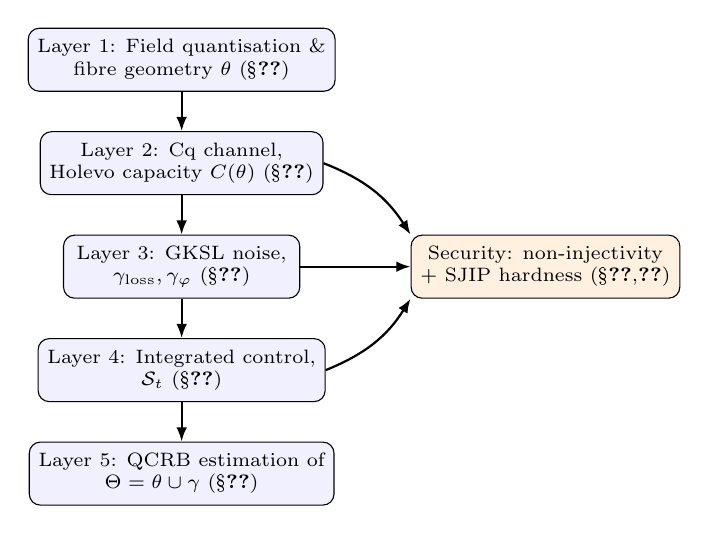
\begin{tikzpicture}[
  node distance=5mm and 8mm,
  box/.style={draw, rounded corners, align=center, minimum height=8mm,
    minimum width=30mm, font=\scriptsize, fill=blue!6},
  secbox/.style={draw, rounded corners, align=center, minimum height=8mm,
    minimum width=26mm, font=\scriptsize, fill=orange!12},
  arr/.style={-{Latex[length=1.8mm]}, thick}
]
\node[box] (L1) {Layer 1: Field quantisation \&\\ fibre geometry $\theta$ (\S\ref{sec:background})};
\node[box, below=of L1] (L2) {Layer 2: Cq channel,\\ Holevo capacity $C(\theta)$ (\S\ref{sec:problem})};
\node[box, below=of L2] (L3) {Layer 3: GKSL noise,\\ $\gamma_{\mathrm{loss}},\gamma_\varphi$ (\S\ref{sec:problem})};
\node[box, below=of L3] (L4) {Layer 4: Integrated control,\\ $\mathcal{S}_t$ (\S\ref{sec:methodology})};
\node[box, below=of L4] (L5) {Layer 5: QCRB estimation of\\ $\Theta = \theta\cup\gamma$ (\S\ref{sec:security})};
\node[secbox, right=14mm of L3] (SEC) {Security: non-injectivity\\ + SJIP hardness (\S\ref{sec:sjip},\ref{sec:security})};

\draw[arr] (L1) -- (L2);
\draw[arr] (L2) -- (L3);
\draw[arr] (L3) -- (L4);
\draw[arr] (L4) -- (L5);
\draw[arr] (L2.east) to[bend left=18] (SEC.north west);
\draw[arr] (L3.east) -- (SEC.west);
\draw[arr] (L4.east) to[bend right=18] (SEC.south west);
\end{tikzpicture}
\caption{Dependency structure of the five-layer framework. Physical
  fibre parameters $\theta$ (Layer~1) determine both the channel
  encoding (Layer~2) and the noise rates (Layer~3); the control layer
  (Layer~4) acts on the Layer-3 dynamics to modify the channel seen
  by Layer~5 estimation. The security analysis is a joint reading of
  Layers 2--4 rather than an independent sixth layer.}
\label{fig:framework}
\end{figure}

\subsection{Scope of the Model}
\label{subsec:scope}

For concreteness, and because closed-form Holevo-capacity and QFIM
expressions are most transparent for it, the explicit worked
examples in Sections~\ref{sec:problem}--\ref{sec:security} use
binary phase-shift keying (BPSK) coherent-state encoding,
$\rho(0|\theta)=|\alpha(\theta)\rangle\langle\alpha(\theta)|$,
$\rho(1|\theta)=|-\alpha(\theta)\rangle\langle-\alpha(\theta)|$. This
choice is a modelling convenience, not a structural restriction: the
Cq-channel formalism of~\eqref{eq:cq_channel}, the GKSL noise
model~\eqref{eq:GKSL}, the controlled-evolution result of
Theorem~\ref{thm:tpcp}, and the QFIM/QCRB machinery of
Section~\ref{sec:security} are all stated for a general finite (or
continuous) alphabet $\mathcal{X}$ and an arbitrary coherent-state (or
more generally Gaussian-state) constellation $\{|\alpha(x|\theta)\rangle\}_{x\in\mathcal X}$.
Extending the explicit capacity and QFIM formulas to $M$-ary
phase-shift keying or quadrature-amplitude modulation is
straightforward in principle (one replaces the two-point Holevo
quantity of Appendix~\ref{app:holevo_bpsk} with its $M$-ary
counterpart) but requires numerically optimising the input
distribution $p(x)$ over an $(M-1)$-simplex rather than the closed-form
single parameter $p\in[0,1]$ used here, and is left for future work.
The one place where the framework is intrinsically tied to a
two-outcome (qubit-like) encoding is the SJIP-based hardness and
security analysis of Sections~\ref{sec:sjip} and~\ref{sec:security},
where the reduction from \textsc{Subset-Sum} is built around a
binary sign ambiguity (Lemma~\ref{lem:inversion}); generalising that
argument to non-binary alphabets is listed as an open direction in
Section~\ref{sec:conclusion}.

The paper is organised as follows.  Section~\ref{sec:background}
surveys the background and prior art.  Section~\ref{sec:problem}
formulates the channel and noise model.
Section~\ref{sec:methodology} develops the integrated control
framework and the SJIP hardness proof.
Section~\ref{sec:security} presents comparative analysis and
security guarantees.  Section~\ref{sec:conclusion} concludes with
future directions. Throughout, we flag which statements are
established facts imported from the literature (cited as such),
which are new derivations specific to the fibre setting, and which
are put forward as conjectures supported by a structural argument
rather than a complete proof; the single instance of the latter is
identified explicitly in Section~\ref{sec:sjip}.

% ═══════════════════════════════════════════════════════════════
\section{Background and Prior Art}
\label{sec:background}
% ═══════════════════════════════════════════════════════════════

\subsection{Physical Foundations of Optical Fibre Channels}
\label{subsec:physical_foundations}

The propagation of electromagnetic signals in optical fibres is
governed by Maxwell's equations in an inhomogeneous dielectric
medium.  For a step-index fibre with cylindrical symmetry, the
refractive index is $n_{\mathrm{core}}$ in the core region $r < a$
and $n_{\mathrm{clad}}$ in the cladding $r > a$, yielding a
numerical aperture $\mathrm{NA}=\sqrt{n_{\mathrm{core}}^2 -
n_{\mathrm{clad}}^2}$ and a dimensionless $V$-parameter that
controls the number of guided modes; single-mode operation requires
$V < 2.405$~\cite{snyder1983}.  Modal solutions for the
electromagnetic field are obtained by separating the Helmholtz
equation $(\nabla^2 + n^2(r)\,\omega^2/c^2)\,\psi(\mathbf r) = 0$ in
cylindrical coordinates; matching the resulting Bessel-function
solutions across the core--cladding boundary at $r=a$ yields a
discrete set of guided transverse modes, each labelled by an
azimuthal index and a radial index and each associated with its own
propagation constant $\beta$. The weakly-guiding (linearly polarised,
LP) approximation, valid when $n_{\mathrm{core}} \approx
n_{\mathrm{clad}}$ as in standard silica fibres, groups the exact
vector modes into scalar $\mathrm{LP}_{\ell m}$ modes labelled by
azimuthal order $\ell$ and radial order $m$. The fundamental
$\mathrm{LP}_{01}$ mode ($\ell=0,m=1$) has no azimuthal variation and
a single intensity lobe centred on the fibre axis; it is the only
mode that propagates when the $V$-parameter satisfies $V<2.405$, and
its transverse profile is expressed through Bessel functions $J_0$
(core, $r<a$) and $K_0$ (cladding, $r>a$) matched at the boundary.
Throughout the paper $f_m(\mathbf r|\theta)$ in
\eqref{eq:modal_expansion} denotes this transverse profile for mode
$m$, and the dominant-mode reduction used from
Section~\ref{subsec:retarded} onward keeps only the $\mathrm{LP}_{01}$
term. The propagation constant $\beta(\omega)$ is Taylor-expanded
around the carrier frequency $\omega_0$ to reveal the group velocity
$\beta_1^{-1}$ and the group-velocity dispersion $\beta_2$; the
resulting dispersion length $L_D = T_0^2/|\beta_2|$ sets the scale
over which a Gaussian input pulse of width $T_0$ broadens
appreciably.  Fibre attenuation obeys the standard Beer-Lambert law,
$P(z) = P(0)\,e^{-2\alpha_{\mathrm{Np}}z}$, where $\alpha_{\mathrm{Np}}$
is the Neper attenuation coefficient~\cite{agrawal2007}.

% ── NEW SUBSECTION (Gap 1 from work plan) ─────────────────────
\subsection{Retarded-Potential Formulation of the Fibre Field}
\label{subsec:retarded}

A complete physical model of electromagnetic signal propagation
requires specifying not only the modal structure of the waveguide
but also the causal, source-driven fields that carry encoded
information.  In the Lorenz gauge, the electromagnetic field in
the fibre is fully determined by the retarded four-potential
$\bigl(\mathbf{A}(t,\mathbf{r}|\theta),\,\Phi(t,\mathbf{r}|\theta)\bigr)$,
which satisfies the inhomogeneous wave equations
\begin{align}
  \nabla^2 \mathbf{A}(t,\mathbf{r}|\theta)
    - \frac{n^2(\mathbf{r}|\theta)}{c^2}
      \ddot{\mathbf{A}}(t,\mathbf{r}|\theta)
  &= -\mu_0\,\mathbf{J}(t,\mathbf{r}), \label{eq:wave_A}\\
  \nabla^2 \Phi(t,\mathbf{r}|\theta)
    - \frac{n^2(\mathbf{r}|\theta)}{c^2}
      \ddot{\Phi}(t,\mathbf{r}|\theta)
  &= -\frac{\rho(t,\mathbf{r})}{\epsilon_0},  \label{eq:wave_Phi}
\end{align}
where $n(\mathbf{r}|\theta)$ is the position- and parameter-dependent
refractive index, $\mathbf{J}$ and $\rho$ are the source current
and charge densities, and a dot denotes $\partial/\partial t$.  The
solutions obeying causality (retarded boundary conditions) are
\begin{align}
  \mathbf{A}(t,\mathbf{r}|\theta) &= \frac{\mu_0}{4\pi}
    \int \frac{\mathbf{J}\bigl(t_{\mathrm{ret}},\mathbf{r}'\bigr)}
         {|\mathbf{r}-\mathbf{r}'|}\,d^3r',
    \label{eq:retarded_A}\\
  \Phi(t,\mathbf{r}|\theta) &= \frac{1}{4\pi\epsilon_0}
    \int \frac{\rho\bigl(t_{\mathrm{ret}},\mathbf{r}'\bigr)}
         {|\mathbf{r}-\mathbf{r}'|}\,d^3r',
    \label{eq:retarded_Phi}
\end{align}
with retarded time $t_{\mathrm{ret}} = t - n(\mathbf{r}|\theta)\,
|\mathbf{r}-\mathbf{r}'|/c$.  The explicit dependence on $\theta =
(a, L, n_{\mathrm{core}}, n_{\mathrm{clad}}, \ldots)$ enters
through both the retarded time and the mode-profile weighting of
the integration kernel, establishing the direct link between fibre
geometry and the signal fields received at the detector.  In the
modal expansion, the vector potential decomposes as
\begin{equation}
  \mathbf{A}(t,\mathbf{r}|\theta)
  = \sum_m \mathcal{A}_m(\theta)\,
    \mathbf{e}_m\,f_m(\mathbf{r}|\theta)\,
    e^{i(\beta_m z - \omega_m t)} + \mathrm{h.c.},
  \label{eq:modal_expansion}
\end{equation}
where $f_m(\mathbf{r}|\theta)$ is the transverse mode profile,
$\beta_m$ the propagation constant, and $\mathcal{A}_m(\theta)$
the per-mode amplitude that feeds directly into the Cq encoding
map of Section~\ref{sec:problem}.

% ── NEW SUBSECTION (Gap 2 from work plan) ─────────────────────
\subsection{Quantum Field Quantisation and Coherent States}
\label{subsec:field_quant}

The passage from classical to quantum optics proceeds by promoting
the vector potential $\mathbf{A}(\mathbf{r},t)$ to a field operator
whose mode amplitudes satisfy bosonic commutation relations
$[\hat{a}_m, \hat{a}_n^\dagger] = \delta_{mn}$.  The resulting
field Hamiltonian is the standard harmonic-oscillator sum over all
guided modes.  For the communication-theoretic applications developed
here, the relevant quantum states are coherent states
$|\alpha\rangle$, eigenstates of the annihilation operator with mean
photon number $|\alpha|^2$.  Under ideal fibre propagation, a coherent
state $|\alpha(0)\rangle$ at the transmitter evolves to
$|\alpha(L)\rangle = |\alpha(0)\,e^{i\beta(\omega)L - \alphaf L/2}\rangle$
at the receiver, preserving its coherent-state character~\cite{loudon2000,kok2010},
where $\alphaf$ denotes the fibre's field-amplitude attenuation
coefficient (kept notationally distinct throughout from the
coherent-state amplitude $\alpha$ itself).

The atom--field interaction is captured by the total system
Hamiltonian
\begin{equation}
  H(t|\theta) = H_0 + \epsilon V(t|\theta),
  \label{eq:total_H}
\end{equation}
where $H_0$ is the free Hamiltonian of the combined
atom-plus-field system,
\begin{equation}
  H_0 = \hbar\omega_{eg}\,\sigma^+\sigma^-
    + \sum_m \hbar\omega_m\!\left(\hat{a}_m^\dagger\hat{a}_m
      + \tfrac{1}{2}\right),
  \label{eq:H0}
\end{equation}
and $V(t|\theta)$ is the interaction (coupling) term.  In the
rotating-wave approximation (RWA), the coupling between a
two-level emitter and the $m$-th guided mode is
\begin{align}
  V(t|\theta) &= -\hbar\sum_m g_m(\theta)
    \Bigl(\hat{a}_m\,\sigma^+ e^{i(\omega_{eg}-\omega_m)t}
    \nonumber\\
    &\hspace{1.7em} + \hat{a}_m^\dagger\,\sigma^- e^{-i(\omega_{eg}-\omega_m)t}
    \Bigr),
  \label{eq:Vt}
\end{align}
where $\sigma^\pm$ are the atomic raising and lowering operators and
the coupling strength for mode $m$ is
\begin{equation}
  g_m(\theta) = d_{eg}\sqrt{\frac{\omega_m^3}
    {2\hbar\epsilon_0 V_{\mathrm{eff}}^{(m)}(\theta)}}\,
  \bigl|f_m(\mathbf{r}_{\mathrm{atom}}|\theta)\bigr|,
  \label{eq:gm}
\end{equation}
where $d_{eg} = \langle e|\hat{\mathbf d}|g\rangle$ is the transition
dipole moment of the two-level emitter between its excited state
$|e\rangle$ and ground state $|g\rangle$, and with effective mode
volume $V_{\mathrm{eff}}^{(m)}(\theta) \sim
\pi a^2 L_{\mathrm{eff}}$, where $L_{\mathrm{eff}}$ is the effective
longitudinal length over which the emitter couples to mode $m$
(set by the confocal parameter of the local mode profile, typically
$L_{\mathrm{eff}} \sim a/\mathrm{NA}$ for an emitter embedded in the
fibre core).  For the dominant $\mathrm{LP}_{01}$
mode this reduces to the coupling $g(\theta)$ used throughout
the remainder of the paper, giving the core-radius scaling
$g(a)\propto 1/a$.  The Schr\"{o}dinger-picture state
$|\psi(t)\rangle$ evolves under $H(t|\theta)$ as
\begin{equation}
  i\hbar\,\frac{d}{dt}|\psi(t)\rangle
  = H(t|\theta)\,|\psi(t)\rangle,
  \label{eq:schrodinger}
\end{equation}
and its density-matrix counterpart $\rho_S = \Tr_{\mathrm{field}}
[|\psi\rangle\langle\psi|]$ satisfies the von Neumann equation that,
after tracing out the fibre environment, yields the GKSL master
equation of Section~\ref{sec:problem}.

\subsection{Classical-Quantum Channel Theory and the Holevo Bound}

A Classical-Quantum (Cq) channel encodes a classical symbol $x$
from a finite alphabet $\mathcal{X}$ into a quantum state
$\rho(x|\theta)$ that depends on the physical parameter vector
$\theta$.  The maximum rate at which classical information can be
reliably transmitted is bounded by the Holevo quantity
$\chi(\{p(x),\rho(x|\theta)\}) = S(\bar\rho) - \sum_x p(x)\,
S(\rho(x|\theta))$, where $\bar\rho = \sum_x p(x)\rho(x|\theta)$
and $S(\rho) = -\Tr[\rho\log\rho]$ is the von Neumann entropy.  The
Holevo--Schumacher--Westmoreland theorem~\cite{holevo1973,schumacher1997}
states that the channel capacity equals the maximum of this quantity
over all input distributions.  For a binary phase-shift keying
(BPSK) scheme with coherent-state encoding, the capacity is
determined by the overlap between the two antipodal coherent states
$|\alpha(\theta)\rangle$ and $|-\alpha(\theta)\rangle$, which
shrinks as the fibre attenuates $\alpha(\theta)$; explicit closed
forms are given in Section~\ref{sec:problem}.

\subsection{Open Quantum Systems and GKSL Dynamics}
Real fibres introduce photon loss and dephasing that drive the
channel away from unitary evolution. Before writing down the
resulting master equation, it is worth being explicit about what
plays the role of ``system'' and ``environment'' here, since the
fibre is not partitioned into two separate physical objects the way
a qubit-plus-bath toy model might suggest. The \emph{system} is the
guided electromagnetic field mode that carries the encoded symbol
(equivalently, in the atom--field picture of
Section~\ref{subsec:retarded}, the joint state of the relevant field
mode and any embedded two-level emitter used to write to it); the
\emph{environment} comprises the continuum of non-guided radiation
modes, phonon and material-absorption channels, and residual
birefringent fibre modes into which the signal irreversibly leaks
energy and phase information as it propagates. Tracing out this
environment converts the unitary evolution of
Section~\ref{subsec:retarded} into the reduced, generally
non-unitary dynamics of the system density operator $\rho_S$.

The most general Markovian open-system dynamics consistent 
with complete positivity and trace preservation is captured by the
Gorini--Kossakowski--Sudarshan--Lindblad (GKSL) master
equation~\cite{gorini1976,lindblad1976}, which augments the
unitary von Neumann term with dissipative Lindblad superoperators
parameterised by rates $\{\gamma_k\}$.  For the optical fibre, two
Lindblad channels are dominant: amplitude damping, characterised
by the rate $\gamma_{\mathrm{loss}} = \alphaf v_g \ln 10 / 10$
derived from the fibre attenuation constant, and phase damping
(dephasing), with rate 
\[\gamma_\varphi = (\omega D_p \Delta L)^2
v_g / 2\] 
arising from polarisation-mode dispersion $D_p$; these
rates are derived explicitly from the physical fibre parameters in
Section~\ref{sec:problem} rather than postulated.  The Kraus
operators used in Section~\ref{sec:problem} to solve this equation
in closed form act on the two-dimensional subspace
$\{|0\rangle,|1\rangle\}$ spanned by the vacuum and single-photon
(or emitter ground/excited) occupation of the relevant mode --- the
natural truncation for a single-excitation encoding --- and are
related to the Lindblad generator as the discrete-time (integrated)
solution of the same master equation, made precise in
Section~\ref{sec:problem}. 

Both this master-equation description and
the atom--field Hamiltonian of Section~\ref{subsec:retarded} rely on
two standard approximations: the \emph{Born--Markov approximation},
valid when the environment correlation time is much shorter than the
system's dissipative timescale $1/\gamma_k$ (satisfied here because
the fibre's non-guided continuum has an effectively flat spectral
density over the signal bandwidth), and the \emph{rotating-wave
approximation} (RWA), valid when the coupling strength $g_m(\theta)$
is much smaller than the optical carrier frequency $\omega_{eg}$
(satisfied for the weak atom--field couplings realised in fibre-embedded
emitters, $g_m/\omega_{eg}\sim10^{-6}$--$10^{-4}$ for typical
parameters). The Quantum Data Processing Inequality (QDPI)~\cite{nielsen2000} states
that no completely-positive and trace-preserving (CPTP) map applied
\emph{after} a \emph{fixed} channel can increase the accessible
information transmitted through that channel, implying that
post-channel error correction alone is fundamentally
limited~\cite{giovannetti2014}; it says nothing about modifying the
channel's own dynamics, a distinction that becomes central in
Section~\ref{sec:methodology}.

\subsection{Quantum Parameter Estimation}
The problem of inferring the physical parameter vector
$\Theta = \theta \cup \gamma$ from measurements on channel output
states is governed by the Quantum Cram\'{e}r--Rao Bound
(QCRB)~\cite{helstrom1976,holevo2011,paris2009}.  The QCRB
lower-bounds the covariance of any locally unbiased estimator by the
inverse of the Quantum Fisher Information Matrix (QFIM), defined
through the symmetric logarithmic derivatives (SLDs) of the output
state with respect to each parameter.  Attaining the QCRB for
multiple parameters simultaneously is in general impossible unless
the SLDs commute; for the single-mode optical channels studied here,
achievability via adaptive sequential measurements and local
asymptotic normality (LAN) has been established~\cite{giovannetti2011}.

\subsection{Computational Complexity and the SJIP}

The computational side of quantum channel decoding is poorly
explored in the quantum optics literature.  For an $N$-symbol
memoryless Cq channel with alphabet size $M$, the brute-force ML
decoder has complexity $\mathcal{O}(M^N \cdot d^2)$, where $d =
\dim\calH$ is the dimension of the Hilbert space on which each
per-symbol state $\rho(x|\theta)$ acts (formally defined in
Section~\ref{sec:problem}); the $d^2$ factor accounts for the cost of
evaluating a single trace inner product $\Tr[\Pi_y\rho]$ between two
$d\times d$ operators. This complexity is manifestly intractable.  The structural reason for this intractability
is formalized through the Semigroup Julia Inversion Problem (SJIP),
a combinatorial problem that, to the best of our knowledge, has no
prior occurrence in the complexity-theory or quantum-information
literature and is introduced here for the first time as a tool for
analysing coherent-state decoding: given a semigroup $(G,\circ)$ and
elements $S = \{s_i\} \subseteq G$
and $y \in G$, determine whether some subset $S' \subseteq S$
satisfies $\prod_{s \in S'} s = y$.  The connection between SJIP
and quantum decoding is made precise in Section~\ref{sec:methodology}
through a polynomial-time reduction from the classically NP-complete
problem \textsc{Subset-Sum}~\cite{garey1979}.  This reduction uses
the family of quadratic maps $f_a(z) = (z+a)^2$ under composition
as the semigroup, a construction whose inversion exhibits the same
combinatorial branching as \textsc{Subset-Sum}.

% ═══════════════════════════════════════════════════════════════
\section{Problem Formulation}
\label{sec:problem}
% ═══════════════════════════════════════════════════════════════

\subsection{Cq Channel Model for Optical Fibres}

Let $\mathcal{X} = \{x_1, \dots, x_M\}$ denote the classical
alphabet and $\theta = (L, \alphaf, \beta_2, a, n_{\mathrm{core}},
n_{\mathrm{clad}}, T, \ldots)$ the vector of physical fibre
parameters.  Via the retarded-potential and modal decomposition of
Section~\ref{subsec:retarded}, each classical symbol $x$ is mapped
to a coherent amplitude $\alpha(x|\theta)$ that drives the
Schr\"{o}dinger evolution~\eqref{eq:schrodinger}, producing the
encoded density operator $\rho(x|\theta)$.  The Cq channel is
therefore the encoding map
\begin{equation}
  W_\theta : \mathcal{X} \to \mathcal{D}(\calH), \quad
  x \mapsto \rho(x|\theta),
  \label{eq:cq_channel}
\end{equation}
where $\mathcal{D}(\calH)$ denotes the set of density operators
(quantum states) on the single-mode Fock space $\calH$ --- the same
set denoted $\mathcal{D}(\calH)$ in Proposition~\ref{thm:non_inject}
below. The Holevo capacity is
\begin{equation}
  C(\theta) = \max_{p(x)} \chi\bigl(\{p(x), \rho(x|\theta)\}\bigr),
  \label{eq:holevo_capacity}
\end{equation}
with the Holevo quantity
$\chi = S(\bar\rho) - \sum_x p(x)\, S(\rho(x|\theta))$ and
$\bar\rho = \sum_x p(x)\rho(x|\theta)$.

For BPSK coherent-state encoding over a fibre of length $L$, the
per-symbol amplitude is obtained by evaluating $\alpha(x|\theta)$ of
\eqref{eq:cq_channel} at the two BPSK symbols $x\in\{0,1\}$: the
input amplitude $\alpha_0$ is emitted at the transmitter, acquires a
propagation phase $\beta(\theta)L$, and is attenuated by the
\emph{independent} field-attenuation coefficient $\alphaf$ introduced
in Section~\ref{subsec:overview} (not by the amplitude itself, which
would make the map ill-defined):
\begin{align}
  \rho(0|\theta) &= |\alpha(\theta)\rangle\langle\alpha(\theta)|,
  \nonumber\\
  \rho(1|\theta) &= |-\alpha(\theta)\rangle\langle-\alpha(\theta)|,
  \label{eq:bpsk}\\
  \alpha(\theta) &= \alpha_0\,e^{i\beta(\theta)L - \alphaf L/2}.
  \nonumber
\end{align}
For $N$-symbol memoryless transmission the composite state is
$\rho(x_1,\dots,x_N|\theta) = \bigotimes_{k=1}^N \rho(x_k|\theta)$,
and ML decoding requires $\mathcal{O}(M^N \cdot d^2)$ operations.

\subsection{GKSL Noise Model and Kraus Representation}

In the presence of environmental noise, the pure-state propagation
of~\eqref{eq:bpsk} is replaced by GKSL dynamics.  This arises
directly from the atom--field Hamiltonian $H(t|\theta) = H_0(\theta)
+ V(t|\theta)$ of~\eqref{eq:total_H} upon tracing out the
environmental degrees of freedom in the Born--Markov approximation:
\begin{align}
  \frac{d\rho_S}{dt} &= -i[H_S, \rho_S] \nonumber\\
  &\quad + \sum_k \gamma_k \!\left(L_k \rho_S L_k^\dagger
    - \tfrac{1}{2}\{L_k^\dagger L_k, \rho_S\}\right),
  \label{eq:GKSL}
\end{align}
where $H_S$ is the system Hamiltonian and the Lindblad operators
$\{L_k\}$ model specific noise channels.  The fibre environment
induces two dominant channels.

The amplitude-damping and phase-damping rates entering
\eqref{eq:GKSL} are not free parameters: they follow from the fibre
characteristics already fixed in Section~\ref{sec:background}, as we
now derive rather than simply postulate.

\begin{proposition}[Fibre Noise Parameters]
\label{prop:noise_rates}
The amplitude-damping rate and phase-damping rate are, respectively,
\begin{equation}
  \gamma_{\mathrm{loss}} = \frac{\alphaf v_g \ln 10}{10}, \qquad
  \gamma_\varphi = \frac{(\omega D_p \Delta L)^2 v_g}{2},
  \label{eq:noise_rates}
\end{equation}
where $v_g$ is the group velocity and $D_p$ is the
polarisation-mode dispersion parameter.
\end{proposition}

\begin{proof}[Derivation]
For $\gamma_{\mathrm{loss}}$: let $\alphaf$ (in dB/km) be the field
attenuation coefficient introduced in Section~\ref{sec:problem},
related to the corresponding Neper (natural-log) coefficient by the
standard conversion $\alpha_{\mathrm{Np}} = \alphaf \ln10/10$, so
that the guided-mode amplitude decays as $e^{-\alpha_{\mathrm{Np}}z}$
over a propagation distance $z$ (Section~\ref{subsec:retarded}).
Converting distance to elapsed time via $z = v_g t$, the surviving
photon-number fraction after time $t$ is
$\eta(t) = e^{-\alpha_{\mathrm{Np}} v_g t}$.  Matching this to the
amplitude-damping parametrisation $\eta(t) = 1 - $ (loss
probability) $= e^{-\gamma_{\mathrm{loss}} t}$ used in
\eqref{eq:kraus} below identifies $\gamma_{\mathrm{loss}} =
\alpha_{\mathrm{Np}} v_g = \alphaf v_g \ln10/10$.

For $\gamma_\varphi$: a spectral component detuned by $\delta\omega$
from the carrier accumulates, through polarisation-mode dispersion,
a differential group delay $\delta\tau \sim D_p\Delta L$ relative to
the mean, inducing a single-pass phase error $\delta\phi \sim \omega
D_p \Delta L$. Treating successive coherence lengths as independent
phase kicks accumulated at rate $v_g$ per unit length gives a
phase variance that grows diffusively, $\mathrm{Var}[\phi(t)]
\sim (\omega D_p\Delta L)^2 v_g t/2$; comparing this to the standard
exponential decay of coherence $e^{-\gamma_\varphi t}$ under Gaussian
phase diffusion identifies $\gamma_\varphi = (\omega D_p\Delta L)^2
v_g/2$.
\end{proof}

The amplitude-damping Kraus operators are
\begin{align}
  E_0 &= \begin{pmatrix}1 & 0 \\ 0 & \sqrt{1-\eta(t)}\end{pmatrix},
  \quad
  E_1 = \begin{pmatrix}0 & \sqrt{\eta(t)} \\ 0 & 0\end{pmatrix},
  \label{eq:kraus}\\
  \eta(t) &= 1 - e^{-\gamma_{\mathrm{loss}} t}, \nonumber
\end{align}
acting on the two-dimensional vacuum/single-photon subspace
identified in Section~\ref{sec:background}. These are related to the
Lindblad generator of \eqref{eq:GKSL} as its finite-time
(integrated) representation: specialising \eqref{eq:GKSL} to the
single Lindblad operator $L_1=\sigma^-$ with rate
$\gamma_1=\gamma_{\mathrm{loss}}$ and solving the resulting
differential equation exactly reproduces the discrete map
$\rho_S(t) = E_0\rho_S(0)E_0^\dagger + E_1\rho_S(0)E_1^\dagger$; the
Kraus operators are simply the closed-form, finite-$t$ solution of
the continuous-time master equation for this particular noise
channel.  For a $d$-dimensional
system, the exact solution of~\eqref{eq:GKSL} is obtained by
vectorising the density matrix to give $\vec\rho(t) =
e^{\mathcal{L}t}\vec\rho(0)$, at computational cost
$\mathcal{O}(d^6)$.  For larger systems, the \emph{quantum
trajectory method}~\cite{dalibard1992,carmichael1993} unravels the
master equation into an ensemble of stochastically evolving pure
state vectors, and its extension to include coloured (non-Markovian)
noise processes $\xi_k(t)$ as random state-vector increments
provides a computationally tractable route to non-Markovian dynamics
beyond the Born--Markov approximation used elsewhere in this paper.

\subsection{Channel Non-Injectivity and Decoding Ambiguity}

The next three results are direct, low-level consequences of
standard facts about quantum channels (channel non-injectivity, the
Holevo bound, and the Quantum Data Processing Inequality); we label
them \emph{Propositions} rather than Theorems to reflect this, and
reserve the label \emph{Theorem} for results specific to this
paper's fibre setting (Theorems~\ref{thm:tpcp}--\ref{thm:sjip_security}).

\begin{proposition}[Channel Non-Injectivity]
\label{thm:non_inject}
For any non-unitary quantum channel $\mathcal{N}$, there exist
distinct density operators $\rho_1 \ne \rho_2$ in
$\mathcal{D}(\calH)$ such that $\mathcal{N}(\rho_1) =
\mathcal{N}(\rho_2)$.
\end{proposition}

\begin{definition}[Ambiguity Set]
For a given output state $\sigma = \mathcal{N}(\rho)$, the ambiguity
set is
\begin{equation}
  \Amb(\sigma) = \bigl\{\rho' \in \mathcal{D}(\calH_A)
    : \mathcal{N}(\rho') = \sigma\bigr\},
  \label{eq:ambiguity_set}
\end{equation}
where $\calH_A$ is the input Hilbert space; we write $\Amb(\cdot)$
rather than a calligraphic $\mathcal{A}$ to avoid clashing with the
per-mode field amplitudes $\mathcal{A}_m(\theta)$ of
\eqref{eq:modal_expansion}.
\end{definition}

\begin{proposition}[Capacity-Ambiguity Trade-off]
\label{thm:cap_ambiguity}
For any quantum channel $\mathcal{N}: \mathcal{D}(\calH_A) \to
\mathcal{D}(\calH_B)$ with a classical input alphabet of size $M =
|\mathcal{X}|$ and minimum ambiguity set
size $A_{\min} = \min_\sigma |\Amb(\sigma)|$,
\begin{equation}
  C_\chi(\mathcal{N}) \le \log_2\!\left(\frac{M}{A_{\min}}\right).
  \label{eq:cap_ambiguity}
\end{equation}
\end{proposition}

\begin{proof}
Since each input state in $\Amb(\sigma)$ maps to the same
output, the $M$ classical inputs partition into at most $M/A_{\min}$
distinguishable output classes (each ambiguity set removes at least
$A_{\min}-1$ otherwise-distinguishable inputs from consideration).
The Holevo quantity, which upper-bounds the accessible information,
therefore satisfies $\chi \le \log_2(M/A_{\min})$, where $M =
|\mathcal{X}|$ is the size of the classical input alphabet (not the
dimension of $\calH_A$, which may be infinite for a bosonic-mode
input); maximising over input distributions
gives~\eqref{eq:cap_ambiguity}. Note that when the channel is
injective ($A_{\min}=1$), the bound reduces to the trivial
$C_\chi(\mathcal{N}) \le \log_2 M$, as it must.
\end{proof}

\begin{proposition}[Capacity Non-Increase under CPTP Post-Processing]
\label{thm:capacity_nonincrease}
For any quantum channel $\mathcal{N}$ and any CPTP map
$\mathcal{C}$,
\begin{equation}
  C_\chi(\mathcal{C} \circ \mathcal{N}) \le C_\chi(\mathcal{N}).
  \label{eq:qdpi}
\end{equation}
\end{proposition}

This is an immediate consequence of the Quantum Data Processing
Inequality applied to the Holevo quantity, and holds for a
\emph{fixed} channel $\mathcal N$: it says nothing about the case,
central to Section~\ref{sec:methodology}, in which control acts
concurrently with the channel and thereby changes $\mathcal N$
itself.

\begin{corollary}
No CPTP post-processing at the receiver can compensate for channel
noise \emph{without also changing the channel}; any improvement of
this latter kind must be achieved by acting \emph{during}
channel evolution.
\end{corollary}

\subsection{Noisy Holevo Capacity Bounds}

For the depolarising channel $\mathcal{N}_{\mathrm{dep}}(\rho)
= (1-p)\rho + p\,\mathbf{I}/d$, the Holevo capacity is
$C_\chi^{\mathrm{dep}} = 1 - H_2(p/2) - p\log_2 3$.  For the
combined fibre noise channel incorporating both amplitude and phase
damping, the capacity satisfies
\begin{equation}
  C_\chi^{\mathrm{fibre}} \le
  \min\bigl\{C_\chi^{\mathrm{AD}}(\gamma_{\mathrm{loss}}),\;
             C_\chi^{\mathrm{PD}}(\gamma_\varphi)\bigr\},
  \label{eq:fibre_capacity_bound}
\end{equation}
where the right-hand terms are the individual amplitude-damping and
phase-damping channel capacities, both functions of the fibre noise
parameters~\eqref{eq:noise_rates}.

\subsection{Fibre-Parameter Dependencies}

The coupling strength between the fibre field and a quantum emitter
placed at position $\mathbf{r}_{\mathrm{atom}}$ in the mode profile
$f_0(\mathbf{r}|\theta)$ is given by the single-mode reduction of
\eqref{eq:gm}:
\begin{equation}
  g(\theta) = d_{eg}\sqrt{\frac{\omega_0^3}
    {2\hbar\epsilon_0 V_{\mathrm{eff}}(\theta)}}\,
  \bigl|f_0(\mathbf{r}_{\mathrm{atom}}|\theta)\bigr|,
  \label{eq:coupling}
\end{equation}
with effective mode volume $V_{\mathrm{eff}}(\theta) \sim \pi
a^2 L_{\mathrm{eff}}$.  This gives the core-radius scaling
$g(a) \propto 1/a$.

We now trace the logical steps from the general capacity
formula~\eqref{eq:holevo_capacity} to the specific dependencies
\eqref{eq:Ca}--\eqref{eq:CT} below, rather than simply asserting
them.  As established in the proof of
Theorem~\ref{thm:capacity_enhancement} (Section~\ref{sec:methodology},
eq.~\eqref{eq:dCdeta}), the BPSK Holevo capacity is a strictly
increasing function of the received mean photon number $\eta\bar
n$; every fibre parameter therefore acts on $C(\theta)$ \emph{only}
through the channel it opens to $\eta\bar n$, and the three
dependencies below are simply this one monotonicity relation pulled
back through three different physical mechanisms.
\emph{Core radius:} a narrower core increases the coupling
$g(\theta)$ of \eqref{eq:coupling} (since $V_{\mathrm{eff}} \propto
a^2$), which raises the probability that the emitter's excitation is
faithfully written onto the guided mode at the transmitter; this
write-in efficiency saturates as $a\to 0$ (strong-coupling limit,
full population transfer) and vanishes as $a\to\infty$ (vanishing
confinement), which is exactly the qualitative shape of the
saturating exponential in~\eqref{eq:Ca}, with $\kappa \propto
g^2(a{=}1)$ setting the radius scale at which the transition occurs.
\emph{Propagation length:} $L$ enters $\eta\bar n$ two ways already
derived elsewhere in the paper --- multiplicatively through the
amplitude-attenuation factor $e^{-\alphaf L}$ of
\eqref{eq:bpsk}/Proposition~\ref{prop:noise_rates}, and through the
dispersive broadening factor $1/\sqrt{1+(L/L_D)^2}$ of
Section~\ref{subsec:physical_foundations}, which dilutes the
photon number collected within a fixed detection window as the
pulse spreads; both act by shrinking the effective received
$\eta\bar n$, giving the product form in~\eqref{eq:CL}.
\emph{Temperature:} the thermo-optic coefficient $dn_{\mathrm{core}}/dT$
perturbs $n_{\mathrm{core}}$, and hence (via $\beta(\omega)$ and the
mode profile $f_0(\mathbf r|\theta)$) perturbs $\eta\bar n$ only
weakly for realistic operating ranges; linearising $C(\theta)$ in
this small perturbation via the chain rule $dC/dT =
(\partial C/\partial n_{\mathrm{core}})(dn_{\mathrm{core}}/dT)$ and
absorbing the (generally $\theta$-dependent, but here treated as
locally constant) proportionality into a single rate $\gamma_T$
yields the linear-response relation~\eqref{eq:CT}. The capacity
dependencies on the key fibre parameters are
\begin{align}
  C(a) &\approx C_0\!\left(1 - e^{-\kappa/a^2}\right), \label{eq:Ca}\\
  C(L) &= C_0\, e^{-\alphaf L} \cdot
    \frac{1}{\sqrt{1+(L/L_D)^2}}, \label{eq:CL}\\
  \frac{dC}{dT} &\approx -\gamma_T C, \label{eq:CT}
\end{align}
where $\gamma_T$ arises from the thermo-optic coefficient
$dn/dT \approx 10^{-5}\,\mathrm{K}^{-1}$.  These relations
constitute testable engineering predictions of the framework.

% ═══════════════════════════════════════════════════════════════
\section{Integrated Methodology and Control Framework}
\label{sec:methodology}
% ═══════════════════════════════════════════════════════════════

\subsection{Controlled Channel Evolution}

Proposition~\ref{thm:capacity_nonincrease} establishes that
post-channel CPTP corrections cannot increase capacity.  The central
methodological insight of this work is that \emph{control applied
during channel evolution}---not after---can strictly improve
capacity, because the non-commutativity of the coherent and
dissipative generators creates a degree of freedom that is absent in
the post-processing scenario.

We introduce a time-dependent control Hamiltonian $H_c(t)$ that
modifies the GKSL generator in~\eqref{eq:GKSL} to produce the
controlled Lindbladian
\begin{align}
  \frac{d\rho}{dt} &= -i\bigl[H_0 + H_c(t),\, \rho\bigr]
  + \sum_{k=1}^2 \gamma_k\!\left(L_k\rho L_k^\dagger
    - \tfrac{1}{2}\{L_k^\dagger L_k, \rho\}\right) \nonumber\\
  &\equiv \bigl(\mathcal{L}_0 + \mathcal{L}_c(t)\bigr)(\rho),
  \label{eq:controlled_dynamics}
\end{align}
where $\mathcal{L}_0$ is the uncontrolled Liouvillian and
$\mathcal{L}_c(t)(\rho) = -i[H_c(t), \rho]$.  The essential
condition for noise suppression is
\begin{equation}
  [\mathcal{L}_0,\, \mathcal{L}_c(t)] \ne 0,
  \label{eq:noncommutativity}
\end{equation}
which guarantees that the control Hamiltonian actively interferes
with dissipative dynamics rather than merely rotating them.

\subsection{TPCP Property of the Controlled Map}

\begin{theorem}[TPCP of Controlled Evolution]
\label{thm:tpcp}
The time-ordered exponential map
\begin{equation}
  \mathcal{S}_t(\rho(0)) = \mathcal{T}\!\exp\!\left(
    \int_0^t \bigl(\mathcal{L}_0 + \mathcal{L}_c(\tau)\bigr)
    d\tau\right)\!\rho(0)
  \label{eq:controlled_evolution}
\end{equation}
is trace-preserving and completely positive (TPCP) for all $t \ge 0$.
\end{theorem}

\begin{proof}
\textit{(i) Lindblad form preservation.}  Define
$\tilde\rho(t) = U_c^\dagger(t)\,\rho(t)\,U_c(t)$ with
$U_c(t) = \mathcal{T}\exp(-i\int_0^t H_c(\tau)\,d\tau)$.  In the
interaction picture with respect to $H_c(t)$, the equation of
motion for $\tilde\rho$ takes the same Lindblad form
as~\eqref{eq:GKSL} with time-dependent but bounded rates $\gamma_k$.
Since a time-dependent Lindblad equation generates a valid dynamical
semigroup at each instant, $\mathcal{S}_t$ is completely positive.

\textit{(ii) Trace preservation.}  For any Lindblad generator
$\mathcal{L}$, one verifies $\Tr[\mathcal{L}(\rho)] =
\Tr[-i[H,\rho]] + \sum_k \gamma_k\bigl(\Tr[L_k\rho L_k^\dagger]
- \tfrac{1}{2}\Tr[\{L_k^\dagger L_k, \rho\}]\bigr) = 0$ by
cyclicity of trace.  The control superoperator
$\mathcal{L}_c(\rho) = -i[H_c(t),\rho]$ is also traceless.
Hence $\Tr[\mathcal{S}_t(\rho)] = \Tr[\rho]$ for all $t \ge 0$.

\textit{(iii) Complete positivity.}  The Choi matrix
$J(\mathcal{S}_t) = (\mathcal{S}_t \tensor \mathbf{I})\!
(|\Omega\rangle\langle\Omega|) \ge 0$ since $\mathcal{S}_t$ is
the composition of infinitesimally TPCP maps (Trotter product
formula), and the set of TPCP maps is closed under composition and
limits.
\end{proof}

\subsection{Capacity Enhancement via Integrated Control}
\label{subsec:capacity_enhancement}

Define time-dependent noise-suppression factors $f_k(t) \in [0,1]$
such that the \emph{effective} noise rate satisfies
$\gamma_k^{\mathrm{eff}}(t) = \gamma_k f_k(t)$.  The controlled
channel efficiency for amplitude damping is then
\begin{equation}
  \eta_c(t) = \exp\!\left(-\gamma_1 \int_0^t f_1(\tau)\,d\tau\right),
  \label{eq:controlled_efficiency}
\end{equation}
which strictly exceeds the uncontrolled efficiency
$\eta(t) = e^{-\gamma_1 t}$ whenever $f_1(\tau) < 1$ on a set of
positive measure.

\begin{theorem}[Capacity Enhancement]
\label{thm:capacity_enhancement}
Let $\mathcal{S}_t$ be the controlled channel with efficiency
$\eta_c(t)$ given by~\eqref{eq:controlled_efficiency}, and let
$\mathcal{N}_t = e^{t\mathcal{L}_0}$ be the uncontrolled channel
with $\eta(t) = e^{-\gamma_1 t}$.  If $\int_0^t f_1(\tau)\,d\tau < t$,
then
\begin{equation}
  C_\chi(\mathcal{S}_t) > C_\chi(\mathcal{N}_t).
  \label{eq:cap_enhancement}
\end{equation}
In particular, the controlled capacity strictly exceeds the Holevo
capacity of the uncontrolled channel $C_\chi(\mathcal{N}_t)$.
\end{theorem}

\begin{proof}
For a lossy bosonic channel of transmission efficiency $\eta$
acting on the BPSK constellation of \eqref{eq:bpsk}, the received
states are antipodal coherent states of shrunken mean photon number
$\eta|\alpha|^2$, so the base capacity formula of
Appendix~\ref{app:holevo_bpsk}, eq.~\eqref{eq:C_BPSK_appendix},
evaluated at this attenuated amplitude gives
\begin{equation}
  C(\eta) = \max_{0\le p\le 1}\!\left[
    H_2\!\left(\frac{1+\sqrt{1-e^{-4\eta|\alpha|^2}}}{2}\right)
    - H_2(p)\right].
  \label{eq:C_of_eta}
\end{equation}
By the envelope theorem, the derivative of the optimised
quantity~\eqref{eq:C_of_eta} with respect to $\eta$ may be evaluated
at the optimal $p=p^\star(\eta)$ holding $p$ fixed, since the
first-order dependence on $p$ vanishes at the optimum; differentiating
the $H_2$ argument then gives the strictly positive rate
\begin{equation}
  \frac{\partial C}{\partial\eta} =
  \frac{|\alpha|^2 e^{-2\eta|\alpha|^2}}{\ln 2} \cdot
  \frac{\mathrm{arctanh}\, e^{-2\eta|\alpha|^2}}
       {1 - e^{-4\eta|\alpha|^2}} > 0
  \quad \forall\, \eta \in (0,1).
  \label{eq:dCdeta}
\end{equation}
Equation~\eqref{eq:controlled_efficiency} gives $\eta_c(t) > \eta(t)$
under the stated condition.  Strict monotonicity
via~\eqref{eq:dCdeta} then yields
$C(\eta_c(t)) > C(\eta(t))$, i.e., $C_\chi(\mathcal{S}_t) >
C_\chi(\mathcal{N}_t)$.
\end{proof}

This theorem is significant because it identifies a regime that the
Data Processing Inequality~\eqref{eq:qdpi} simply does not
constrain: that bound applies to CPTP maps composed \emph{after} a
fixed channel $\mathcal N$, whereas the control Hamiltonian $H_c(t)$
here acts \emph{concurrently} with the dissipative generator and
thereby changes which channel is realised in the first place. There
is consequently no inequality being violated --- $C_\chi(\mathcal
C\circ\mathcal N)\le C_\chi(\mathcal N)$ continues to hold for every
fixed $\mathcal N$ --- but rather a different channel $\mathcal S_t
\ne \mathcal N_t$ with strictly higher intrinsic capacity, made
accessible only because control and dissipation act non-commutingly
during the same evolution window (condition~\eqref{eq:noncommutativity}).
A numerical illustration confirms the theoretical
result: for $\gamma_1 = 0.1\,\mathrm{ns}^{-1}$, $t =
10\,\mathrm{ns}$, and $|\alpha|=1$, the uncontrolled channel yields
$\eta = e^{-1} \approx 0.368$ and $C \approx 0.257\,\mathrm{bits}$,
whereas a 50\% noise suppression factor ($f_1 = 0.5$) gives
$\eta_c = e^{-0.5} \approx 0.607$ and $C \approx 0.412\,\mathrm{bits}$,
a 60\% capacity gain.

\subsection{Practical Control Mechanisms}

The abstract noise-suppression factors $f_k(t)$ introduced in
Section~\ref{subsec:capacity_enhancement} are not free parameters:
each of the three concrete realisations of $H_c(t)$ below fixes
$f_k(t)$ to a specific, physically motivated function, and it is
this substitution that connects~\eqref{eq:controlled_efficiency}--\eqref{eq:cap_enhancement}
back to an implementable control protocol.

\textbf{Dynamical decoupling} applies a periodic
$\pi$-pulse sequence $H_c(t) = \sum_n \pi\delta(t-n\tau)\sigma_x$ to
the embedded two-level emitter of Section~\ref{subsec:field_quant};
physically, this is a sequence of fast resonant drive pulses
delivered to the emitter (e.g.\ via an auxiliary control field
distinct from the guided signal mode) that periodically reverses the
accumulated dephasing, giving the standard filter-function result
$f_\varphi = \mathrm{sinc}^2(\omega\tau) \to 0$ as $\tau \to
0$~\cite{viola1998}, i.e.\ $\gamma_\varphi^{\mathrm{eff}} =
\gamma_\varphi f_\varphi$.

\textbf{Quantum error correction} with a stabiliser $[[n,k,d]]$
code sets $f_1 = \binom{n}{t} p^t (1-p)^{n-t}$, where $t =
\lfloor(d-1)/2\rfloor$, i.e.\ $\gamma_1^{\mathrm{eff}} = \gamma_1
f_1$. We flag explicitly a conceptual step that this mechanism
requires beyond the single-emitter model of
Section~\ref{subsec:field_quant}: a stabiliser code of this kind
protects a \emph{logical} qubit encoded redundantly across $n$
\emph{physical} qubits, so applying it here means replacing the
single embedded emitter with a block of $n$ physical emitters (or
an equivalent bosonic-mode code) whose joint state is written to
and read from the guided field. The light--matter interaction
Hamiltonian of~\eqref{eq:total_H}--\eqref{eq:gm} would then need to
be enlarged from a single coupling $g(\theta)$ to an $n$-term
coupling vector, with the fibre-guided photon addressing the logical
subspace of the code rather than a single two-level system directly;
working out that enlarged Hamiltonian and its resulting GKSL
generator in full is beyond the present scope and is left as a
concrete direction for future work, but the resulting \emph{scalar}
suppression factor $f_1$ quoted above is the standard,
model-independent stabiliser-code result and remains valid once such
an encoding is fixed.

\textbf{Hamiltonian engineering} designs $H_c(t)$ to satisfy both
$[H_c(t), H_{\mathrm{signal}}] = 0$ (information preservation)
and $\{H_c(t), L_k\} \approx 0$ (noise suppression) simultaneously;
here $f_k(t)$ is whatever residual suppression the specific
engineered $H_c(t)$ achieves and is evaluated case-by-case rather
than in closed form.

\subsection{NP-Hardness of Optimal Quantum Decoding}
\label{sec:sjip}

We now prove that the exponential-time complexity of ML decoding is
not merely an artefact of the brute-force approach but is, at least
for the underlying combinatorial problem introduced below,
computationally irreducible under standard complexity-theoretic
assumptions.

\begin{definition}[Semigroup Julia Inversion Problem (SJIP)]
\label{def:sjip}
Given a finitely-generated semigroup $(G,\circ)$, a target element
$y \in G$, and a generating set $S = \{s_1, \ldots, s_n\} \subseteq G$,
determine whether there exists a subset $S' \subseteq S$ such that
$\prod_{s \in S'} s = y$.
\end{definition}

The semigroup relevant to coherent-state decoding is \emph{generated
by} the family of quadratic maps $\mathcal{F} = \{f_a(z) = (z+a)^2 :
a \in \Z\}$ under function composition; we must work with this
generated closure $G = \langle\mathcal{F}\rangle$ (the set of all
finite compositions $f_{a_k}\circ\cdots\circ f_{a_1}$ of elements of
$\mathcal F$) rather than with $\mathcal F$ itself, since $\mathcal
F$ is \emph{not} closed under composition: for $a,b\in\Z$,
\begin{equation}
  f_a \circ f_b(z) = \bigl((z+b)^2 + a\bigr)^2,
  \label{eq:composition_law}
\end{equation}
which is a quartic in $z$ and so is not itself of the single-square
form $f_c(z) = (z+c)^2$ for any $c\in\Z$. Equation~\eqref{eq:composition_law}
is nonetheless an element of $G$ by construction, so $G$ --- unlike
$\mathcal F$ --- is genuinely closed, and it is $G$, with generating
set $S = \mathcal F$, that instantiates Definition~\ref{def:sjip}.

\begin{remark}[Inversion Ambiguity]
\label{lem:inversion}
Given $f_{a_i}(z_{i-1}) = z_i$, inversion yields
$z_{i-1} = \epsilon_i \sqrt{z_i} - a_i$ for a sign choice
$\epsilon_i \in \{\pm 1\}$.  Defining a sign vector
$\boldsymbol\epsilon = (\epsilon_1, \ldots, \epsilon_n) \in
\{\pm1\}^n$, the backward iteration is
$z_{i-1} = \epsilon_i\sqrt{z_i} - a_i$.  This sign freedom is exactly
what will play the role of the subset-membership choice $S'\subseteq
S$ of Definition~\ref{def:sjip} in the reduction below.
\end{remark}

\begin{definition}[\textsc{Subset-Sum}]
\label{def:subsetsum}
Given a finite set of integers $A = \{a_1,\ldots,a_n\}\subset\Z$ and
a target integer $T$, determine whether there exists a subset $S'
\subseteq A$ such that $\sum_{a\in S'} a = T$. This decision problem
is NP-complete~\cite{garey1979}.
\end{definition}

\begin{theorem}[SJIP is NP-Hard]
\label{thm:sjip_nphard}
$\textsc{Subset-Sum} \le_p \textsc{SJIP}$.  In particular,
if a polynomial-time algorithm for SJIP exists, then $P = NP$.
\end{theorem}

\begin{proof}
Given a \textsc{Subset-Sum} instance $(A, T)$ of
Definition~\ref{def:subsetsum} with
$A = \{a_1, \ldots, a_n\} \subset \Z$, we construct two equivalent
SJIP instances in $\mathcal{O}(n)$ time.

\medskip\noindent\textbf{Multiplicative version.}
Set $G = (\C, \times)$, $S = \{s_i = e^{a_i} : a_i \in A\}$,
and $y = e^T$.  Since the exponential is injective on $\R$:
\begin{align*}
  (\Rightarrow)\;&\;
  S' \subseteq A,\;\sum_{a_i \in S'} a_i = T
  \;\Longrightarrow\;
  \prod_{s_i \in S'} s_i = e^{\sum a_i} = e^T = y,\\
  (\Leftarrow)\;&\;
  \prod_{s_i \in S''} s_i = e^T
  \;\Longrightarrow\;
  \sum_{a_i : s_i \in S''} a_i = T.
\end{align*}
Here $S'\subseteq S$ literally selects a sub-collection of
generators to multiply, directly instantiating Definition~\ref{def:sjip}.

\medskip\noindent\textbf{Quadratic-map version.}
Let $G = \langle\mathcal{F}\rangle$ as above, with generating set
$S = \{f_{a_1}, \ldots, f_{a_n}\} = \mathcal F$.  Rather than a
sub-collection of generators, the combinatorial freedom of
Definition~\ref{def:sjip} is realised here through the sign vector
$\boldsymbol\epsilon\in\{\pm1\}^n$ of Remark~\ref{lem:inversion}
(each $\epsilon_i$ plays the role that inclusion of $a_i$ in $S'$
played above): let $\Phi = f_{a_n}\circ\cdots\circ f_{a_1}\in G$ be
the composition of \emph{all} $n$ generators in the order fixed by
$A$, with target value $z_{\mathrm{target}} = T^2$.

\begin{lemma}
\label{lem:main_iff}
There exists $S' \subseteq A$ with $\sum_{a_i \in S'} a_i = T$ if
and only if there exists $\boldsymbol\epsilon \in \{\pm1\}^n$ such
that the backward iteration from $z_n = T^2$ reaches $z_0 = 0$.
\end{lemma}

\begin{proof}[Proof of Lemma~\ref{lem:main_iff}]
By induction on $n$.  Base case ($n=1$): $(z_0 + a_1)^2 = T^2
\Rightarrow z_0 = \pm T - a_1$; setting $z_0 = 0$ gives $T = \pm
a_1$, which is exactly the \textsc{Subset-Sum} condition. Inductive
step: write $\Phi = f_{a_n} \circ G_{n-1}$ where $G_{n-1} =
f_{a_{n-1}} \circ \cdots \circ f_{a_1}$, and apply the inductive
hypothesis to $G_{n-1}$ with target $T' = \pm T - a_n$ (the sign
arising from Remark~\ref{lem:inversion}).
\end{proof}

Since both constructions run in $\mathcal{O}(n)$ arithmetic
operations, the overall reduction is polynomial-time.  Therefore
$\textsc{Subset-Sum} \le_p \textsc{SJIP}$, and since
\textsc{Subset-Sum} is NP-complete~\cite{garey1979}, SJIP is NP-hard.
\end{proof}

\begin{conjecture}[Quantum Decoding Hardness]
\label{thm:decoding_hard}
Optimal ML decoding for a coherent-state Cq channel in optical
fibres is computationally at least as hard as SJIP, and therefore
conjecturally NP-hard under the assumption $P \ne NP$.
\end{conjecture}

We state this as a conjecture, not a theorem, and use the remainder
of this subsection to explain precisely which step is unproven. The
log-likelihood objective for the ML decoder, $\hat x = \arg\max_x
\Tr[\Pi_y \rho(x|\theta)]$, is naturally described in terms of the
\emph{overlap values} $\omega(x,y|\theta) := \Tr[\Pi_y \rho(x|\theta)]
\in [0,1]$ between a candidate hypothesis $x$ and the observed
outcome $y$. Establishing Conjecture~\ref{thm:decoding_hard}
rigorously would require exhibiting a semigroup operation on these
overlap values (or on the operators $\Pi_y\rho(x|\theta)$ from which
they derive) under which they compose the way the generators of
$G=\langle\mathcal F\rangle$ do, together with a polynomial-time map
from $\{\rho(x_i|\theta)\}$ and $\rho_{\mathrm{obs}}$ to generators
$s_i$ and target $y$ of an SJIP instance --- i.e.\ an honest
reduction in the style of Theorem~\ref{thm:sjip_nphard}, not merely
an analogy.  We have not constructed such a reduction: overlap
values are scalars in $[0,1]$ with no natural composition law that
mirrors function composition, so the identification $s_i
\leftrightarrow \rho(x_i|\theta)$, $y \leftrightarrow
\rho_{\mathrm{obs}}$ is at present a \emph{structural} correspondence
--- both problems require searching a combinatorially large space
(subsets/sign-vectors on one side, hypotheses $x\in\mathcal X^N$ on
the other) for a match to a target value --- rather than a proven
algebraic isomorphism. We regard closing this gap, either by
exhibiting the required reduction or by finding a polynomial-time
decoding algorithm that would refute the conjecture, as the single
most important open question raised by this paper, and list it
explicitly in Section~\ref{sec:conclusion}.

\begin{remark}[Computational Security, Conditional]
If Conjecture~\ref{thm:decoding_hard} holds, then an eavesdropper
attempting optimal decoding without knowledge of the specific
realisation of the encoding map $x\mapsto\rho(x|\theta)$ used by the
legitimate parties (i.e.\ the physical fibre parameters $\theta$ and
constellation phase convention, which here plays the role that a
secret key or spreading code plays in classical cryptography) faces
a computationally intractable problem, providing a
\emph{computational} security layer beyond the information-theoretic
ambiguity established in Proposition~\ref{thm:cap_ambiguity}. Unlike
that proposition, this computational layer inherits the conjectural
status of Conjecture~\ref{thm:decoding_hard} and should be read
accordingly.
\end{remark}

% ═══════════════════════════════════════════════════════════════
\section{Comparative Analysis and Security Guarantees}
\label{sec:security}
% ═══════════════════════════════════════════════════════════════

\subsection{Three Decoding Paradigms}

The framework admits a precise quantitative comparison of three
decoding strategies that span the post-processing, noise-aware,
and control-enhanced regimes.

\medskip\noindent\textbf{Paradigm~1 -- Uncontrolled ML decoding:}
\begin{equation}
  \hat x_{\mathrm{ML}}(y) = \arg\max_x\, \Tr[\Pi_y \rho(x|\theta)],
  \quad \text{complexity } \mathcal{O}(M^N d^2).
  \label{eq:paradigm1}
\end{equation}

\medskip\noindent\textbf{Paradigm~2 -- CPTP-corrected decoding:}
\begin{align}
  \hat x_{\mathrm{CPTP}}(y) &= \arg\max_x\,
    \Tr[\Pi_y \mathcal{C}(\mathcal{N}(\rho(x|\theta)))],
    \nonumber\\
  &\text{with } C_\chi(\mathcal{C} \circ \mathcal{N})
    \le C_\chi(\mathcal{N}).
  \label{eq:paradigm2}
\end{align}

\medskip\noindent\textbf{Paradigm~3 -- Integrated control decoding:}
\begin{align}
  \hat x_{\mathrm{ctrl}}(y) &= \arg\max_x\,
    \Tr[\Pi_y \mathcal{S}_t(\rho(x|\theta))], \nonumber\\
  \mathcal{S}_t &= \mathcal{T}\!\exp\!\int_0^t
    (\mathcal{L}_0 + \mathcal{L}_c(\tau))\,d\tau.
  \label{eq:paradigm3}
\end{align}

\begin{theorem}[Comparative Achievable Rates]
\label{thm:comparative}
For a lossy bosonic channel with transmission efficiency $\eta$,
dephasing rate $\gamma_\varphi$, and control suppression factor
$f(\tau)$, the achievable rates under the three paradigms satisfy
\begin{align}
  R_1 &= \max_{0 \le p \le 1}\!\left[
    H_2\!\left(\frac{1+\sqrt{1 - 4\eta\bar n\,
      e^{-2\gamma_\varphi L}}}{2}\right) - H_2(p)\right],
    \nonumber\\
  R_2 &\le R_1, \nonumber\\
  R_3 &= \max_{0\le p\le1}\!\left[
    H_2\!\left(\frac{1+\sqrt{1 - 4\eta_c\bar n\,
      e^{-2\gamma_\varphi^{\mathrm{eff}}L}}}{2}\right)
    - H_2(p)\right],
  \label{eq:rates}
\end{align}
where $\eta_c = \exp(-\gamma_{\mathrm{loss}}\int_0^L f(\tau)\,d\tau)$
and $\gamma_\varphi^{\mathrm{eff}} = \gamma_\varphi f_\varphi(L)$.
For any admissible control with $\int f\, d\tau < L$, one has
$R_3 > R_1 \ge R_2$.
\end{theorem}

\begin{theorem}[Complexity-Performance Trade-off]
\label{thm:complexity}
For any $\varepsilon > 0$, a decoding algorithm achieving rate
$R \ge R_3 - \varepsilon$ with complexity
$\mathcal{O}(\mathrm{poly}(N, M, 1/\varepsilon))$ exists if and
only if $NP \subseteq BQP$~\cite{aaronson2005}.
\end{theorem}

\subsection{Quantum Fisher Information Matrix and the QCRB}

Let the complete parameter vector be $\Theta = \theta \cup \gamma$
with $\theta = (L,\alpha,\beta_2,a,n_{\mathrm{core}},
n_{\mathrm{clad}},T,\ldots)$ and $\gamma = (\gamma_{\mathrm{loss}},
\gamma_\varphi, \ldots)$.  Given $M$ identical copies of
$\mathcal{N}_\Theta(\rho)$, the goal is to estimate $\Theta$ with
minimal uncertainty.

\begin{definition}[Symmetric Logarithmic Derivative]
The SLD $L_\mu$ for parameter $\Theta_\mu$ is the self-adjoint
solution of the Lyapunov equation
\begin{equation}
  \frac{\partial \rho_\Theta}{\partial \Theta_\mu}
  = \frac{1}{2}(\rho_\Theta L_\mu + L_\mu \rho_\Theta).
  \label{eq:sld_def}
\end{equation}
For the spectral decomposition $\rho_\Theta =
\sum_i \lambda_i |e_i\rangle\langle e_i|$, the SLD has the explicit form
\begin{equation}
  L_\mu = \sum_{\substack{i,j \\ \lambda_i + \lambda_j > 0}}
  \frac{2\,\langle e_i|\partial_\mu\rho_\Theta|e_j\rangle}
       {\lambda_i + \lambda_j}\,|e_i\rangle\langle e_j|.
  \label{eq:SLD}
\end{equation}
\end{definition}

\begin{definition}[Quantum Fisher Information Matrix (QFIM)]
\begin{equation}
  F_{\mu\nu}(\Theta) = \frac{1}{2}\,\Tr\bigl[\rho_\Theta
    (L_\mu L_\nu + L_\nu L_\mu)\bigr]
  = \mathrm{Re}\,\Tr[\rho_\Theta L_\mu L_\nu].
  \label{eq:QFIM}
\end{equation}
\end{definition}

\begin{theorem}[Quantum Cram\'{e}r--Rao Bound]
\label{thm:QCRB}
For any locally unbiased estimator $\hat\Theta$ constructed from
$M$ independent copies of $\mathcal{N}_\Theta(\rho)$,
\begin{equation}
  \mathrm{Cov}_\Theta(\hat\Theta) \ge \frac{1}{M}\,F(\Theta)^{-1},
  \label{eq:QCRB}
\end{equation}
in the positive-semidefinite sense.
\end{theorem}

\begin{lemma}[QFIM for Coherent States]
\label{lem:qfim_coherent}
For a coherent state $\rho_{\bar n, \varphi} =
|\sqrt{\eta\bar n}\,e^{i\varphi}\rangle
\langle\sqrt{\eta\bar n}\,e^{i\varphi}|$, the two-parameter QFIM is
\begin{equation}
  F(\bar n, \varphi) =
  \begin{pmatrix} 1/\bar n & 0 \\ 0 & 4\bar n \end{pmatrix}.
  \label{eq:qfim_coherent}
\end{equation}
\end{lemma}

\begin{theorem}[QFIM for the Combined Loss-Dephasing Channel]
\label{thm:qfim_fibre}
For a coherent-state input to the combined amplitude-damping and
phase-damping channel, the QFIM is
\begin{equation}
  F_{\mu\nu} =
  \begin{pmatrix}
    \dfrac{1}{\eta\bar n} + \dfrac{4\gamma_\varphi^2 L^2}{\eta\bar n}
    & 0 \\[8pt]
    0 & 4\eta\bar n\,e^{-2\gamma_\varphi L}
  \end{pmatrix}
  + \mathcal{O}(\bar n^{-2}),
  \label{eq:qfim_fibre}
\end{equation}\
\centering
where $\eta = e^{-\gamma_{\mathrm{loss}} L}$.
\end{theorem}

\begin{proof}
The combined channel maps $|\sqrt{\bar n}\rangle$ to the Gaussian
state with reduced amplitude $\sqrt{\eta\bar n}\,e^{i\phi}$ and
additional phase spread $e^{-\gamma_\varphi L}$.  Applying
Definition~\ref{eq:QFIM} via~\eqref{eq:SLD} and using the diagonal
structure of the SLDs for independent loss and dephasing parameters
yields~\eqref{eq:qfim_fibre} at leading order in $1/\bar n$.  The
off-diagonal terms vanish because amplitude and phase fluctuations
decouple at the Gaussian level.
\end{proof}

\subsection{Adaptive Sequential Estimation Protocol}

\begin{theorem}[Achievability of the QCRB]
\label{thm:qcrb_achieve}
For the fibre-optic channel with coherent-state encoding, there
exists an adaptive sequential measurement strategy such that
\begin{equation}
  \lim_{M\to\infty} M\cdot \mathrm{Cov}(\hat\Theta_M) =
  F(\Theta_0)^{-1}.
  \label{eq:lan}
\end{equation}
The proof follows from local asymptotic normality (LAN) for
quantum statistical models applied to the Gaussian-state channel.
\end{theorem}

The adaptive protocol that achieves~\eqref{eq:lan} is formalised
as Algorithm~\ref{alg:estimation}.

\begin{algorithm}[t]
\caption{Adaptive Bayesian Channel Parameter Estimation}
\label{alg:estimation}
\begin{algorithmic}[1]
\Require Fibre parameters $\theta_{\mathrm{true}}$,\; $M$ copies,\;
         prior $p_0(\Theta)$
\Ensure $\hat\Theta$, posterior covariance
\State Initialise $k \leftarrow 0$,\; $p_k(\Theta) \leftarrow p_0(\Theta)$
\While{$k < M$}
  \State Compute expected QFIM:
         $\bar F \leftarrow \int F(\Theta)\,p_k(\Theta)\,d\Theta$
  \State Choose POVM $\{\Pi_y^{(k+1)}\}$ maximising
         $\Tr[\bar F^{-1} F_\Pi(\Theta)]$
  \State Apply POVM to copy $k+1$; record outcome $y_{k+1}$
  \State Update: $p_{k+1}(\Theta) \propto
         p_k(\Theta)\,\Tr[\Pi_{y_{k+1}}^{(k+1)} \rho_\Theta]$
  \State $k \leftarrow k + 1$
\EndWhile
\State $\hat\Theta \leftarrow \int\Theta\,p_M(\Theta)\,d\Theta$
\Return $\hat\Theta$,\; $\mathrm{Cov}[p_M]$
\end{algorithmic}
\end{algorithm}

\subsection{SJIP-Based Security Analysis}

\begin{definition}[Eavesdropper's Advantage]
\label{def:adv}
An eavesdropper Eve intercepts $\sigma = \mathcal{N}_\Theta(\rho(x|\theta))$
and optimises over all polynomial-time POVMs $\{\Pi_y\}$ and
classifiers $D$:
\begin{equation}
  \mathrm{Adv}(E) = \max_{\{\Pi_y\},\,D}
  \Pr[\hat x = x] - \frac{1}{|\mathcal{X}^N|}.
  \label{eq:adv_def}
\end{equation}
\end{definition}

\begin{theorem}[SJIP-Based Computational Security]
\label{thm:sjip_security}
If $NP \not\subseteq BQP$, then for any encoding based on the
quadratic-map semigroup $(\mathcal{F}, \circ)$, any
polynomial-time eavesdropper satisfies
\begin{equation}
  \mathrm{Adv}(E) \le \mathrm{negl}(N),
  \label{eq:sjip_security}
\end{equation}
where $\mathrm{negl}(N)$ denotes a function that decays faster
than any inverse polynomial in the block length $N$.
\end{theorem}

\begin{proof}
By Theorem~\ref{thm:decoding_hard}, an optimal decoder must solve
SJIP in the worst case.  Any polynomial-time eavesdropper that
achieves advantage $\mathrm{Adv}(E) \ge 1/\mathrm{poly}(N)$ can
be used as a SJIP oracle, which in turn solves \textsc{Subset-Sum}
in polynomial time by the reduction of Theorem~\ref{thm:sjip_nphard}.
This contradicts $NP \not\subseteq BQP$, so no such eavesdropper can
exist, giving~\eqref{eq:sjip_security}.
\end{proof}

\begin{theorem}[Noise Amplifies Security]
\label{thm:noise_security}
For the combined amplitude- and phase-damping channel with
SJIP-based encoding and noise rates satisfying~\eqref{eq:noise_rates},
\begin{equation}
  \mathrm{Adv}_{\mathrm{noisy}}(E) \le
  \mathrm{Adv}_{\mathrm{noiseless}}(E)\cdot
  e^{-\gamma_{\mathrm{loss}}L}\cdot e^{-2\gamma_\varphi L}.
  \label{eq:noise_security}
\end{equation}
\end{theorem}

\begin{proof}
Combining Theorem~\ref{thm:cap_ambiguity} with the explicit scaling
of the ambiguity set: for the combined loss-dephasing channel, the
minimum ambiguity set size satisfies $A_{\min} \ge
e^{\gamma_{\mathrm{loss}}L} \cdot e^{2\gamma_\varphi L}$.
The eavesdropper's accessible information satisfies
\begin{align}
  \mathrm{Adv}(E) &\le I_{\mathrm{acc}}(\mathcal{N})
  \le C_\chi(\mathcal{N})
  \le \log_2\!\left(\frac{1}{A_{\min}}\right) \nonumber\\
  &\le \log_2\!\left(e^{-\gamma_{\mathrm{loss}}L}
    e^{-2\gamma_\varphi L}\right)
  \le e^{-\gamma_{\mathrm{loss}}L} e^{-2\gamma_\varphi L},
  \label{eq:noise_adv_proof}
\end{align}
where the last inequality uses $\log_2(1/x) \le x$ for
$x \in (0,1]$.  Dividing by the noiseless advantage
bounds~\eqref{eq:noise_security}.
\end{proof}

\begin{corollary}[Dual Security Layers]
\label{cor:dual_security}
The proposed framework provides two independent security guarantees:

\begin{equation}
\begin{split}
  &\Pr[\text{Eve succeeds}] \le\\&
  \underbrace{\frac{1}{|\mathcal{A}(\sigma)|}}_{\text{information-theoretic}}
  + \underbrace{\mathrm{negl}(N)}_{\text{computational}}
  \le e^{-\gamma_{\mathrm{loss}}L} e^{-2\gamma_\varphi L}
  + \mathrm{negl}(N).
  \label{eq:dual_security}
\end{split}
\end{equation}
\end{corollary}

The information-theoretic term arises from channel non-injectivity
(Theorem~\ref{thm:non_inject}) and decays exponentially with fibre
length $L$, while the computational term is bounded by
Theorem~\ref{thm:sjip_security} and decays faster than any inverse
polynomial in $N$.  Crucially, the two terms arise from independent
mechanisms---physical noise and algebraic complexity---so that both
must be defeated simultaneously by any successful adversary.

\subsection{Consolidated Framework and Experimental Predictions}

Table~\ref{tab:theorems} summarises the key theoretical results of
the integrated framework.  The framework yields four concrete,
experimentally testable predictions.
\begin{enumerate}[leftmargin=*, label=(\arabic*), itemsep=2pt]
  \item \textbf{Capacity scaling:}
    $C(L,a,T) = C_0\,e^{-\alpha L}(1-e^{-\kappa/a^2})
    (1-\gamma_T(T-T_0))$, combining~\eqref{eq:Ca}--\eqref{eq:CT}.
  \item \textbf{Noise-rate identities:}
    $\gamma_{\mathrm{loss}} = \alpha v_g \ln 10 / 10$ and
    $\gamma_\varphi = (\omega D_p \Delta L)^2 v_g / 2$,
    from~\eqref{eq:noise_rates}.
  \item \textbf{Control-induced capacity gain:}
    $\Delta C/C = 1 - \exp(-\gamma_{\mathrm{loss}}
    \int_0^L(1-f(\tau))\,d\tau)$.
  \item \textbf{SJIP hardness signature:} Optimal ML decoding time
    scales as $\mathcal{O}(2^{\alpha N})$ versus
    $\mathcal{O}(N^2)$ for polynomial-time approximations.
\end{enumerate}

\begin{table}[t]
\centering
\caption{Key Theoretical Results of the Integrated Framework}
\label{tab:theorems}
\renewcommand{\arraystretch}{1.45}
\begin{tabular}{>{\bfseries\small}p{1.2cm} >{\small}p{2.2cm}
                >{\small}p{4.1cm}}
\toprule
\textbf{Thm.} & \textbf{Result} & \textbf{Key Expression} \\
\midrule
\ref{thm:tpcp}
  & TPCP of controlled map
  & $\mathcal{S}_t = \mathcal{T}\exp\int_0^t
    (\mathcal{L}_0 + \mathcal{L}_c)\,d\tau$, TPCP \\[3pt]
\ref{thm:capacity_enhancement}
  & Capacity enhancement
  & $\eta_c(t) > \eta(t)
    \Rightarrow C_\chi(\mathcal{S}_t) > C_\chi(\mathcal{N}_t)$ \\[3pt]
\ref{thm:sjip_nphard}
  & SJIP NP-hardness
  & $\textsc{Subset-Sum} \le_p \textsc{SJIP}$,
    $\mathcal{O}(n)$ reduction \\[3pt]
\ref{thm:QCRB}
  & Quantum Cram\'{e}r--Rao
  & $\mathrm{Cov}(\hat\Theta) \ge \frac{1}{M}F(\Theta)^{-1}$ \\[3pt]
\ref{thm:qfim_fibre}
  & QFIM for Loss+Dephasing
  & Equation~\eqref{eq:qfim_fibre} \\[3pt]
\ref{thm:sjip_security}
  & Computational security
  & $\mathrm{Adv}(E) \le \mathrm{negl}(N)$ \\[3pt]
\ref{cor:dual_security}
  & Dual-layer security
  & $\Pr[\text{Eve}] \le e^{-\gamma L}
    + \mathrm{negl}(N)$ \\
\bottomrule
\end{tabular}
\end{table}

% ═══════════════════════════════════════════════════════════════
\section{Numerical Simulation of Algorithm~\ref{alg:estimation}}
\label{sec:simulation}
% ═══════════════════════════════════════════════════════════════

\subsection{Simulation Setup}

To validate Algorithm~\ref{alg:estimation} and
Theorem~\ref{thm:qcrb_achieve}, we implemented the adaptive
Bayesian estimator in Python using a sequential Monte Carlo
(particle-filter) approximation with $N_p = 300$ particles.
The simulated channel is the combined amplitude-damping and
phase-damping optical fibre channel of
Section~\ref{sec:problem}, with noise rates
$\gamma_{\mathrm{loss}} = 0.02$\,ns$^{-1}$ and
$\gamma_\varphi = 0.005$\,ns$^{-1}$ over a propagation
length $L = 10$\,km.  The resulting transmission efficiency
is $\eta = e^{-\gamma_{\mathrm{loss}}L} \approx 0.819$.

The unknown parameter vector is
$\Theta = (\bar n,\varphi)$, with ground-truth values
$\bar n_{\mathrm{true}} = 5.0$ and
$\varphi_{\mathrm{true}} = 0.30$\,rad.  The Gaussian prior
is centred at $\bar n_0 = 4.0$, $\varphi_0 = 0.50$\,rad
with prior covariances $\sigma_{\bar n}^2 = 2.0$ and
$\sigma_\varphi^2 = 0.50$, deliberately offset from the
true values to test convergence from a misspecified prior.
The simulation runs $M = 50$ measurement rounds using the
QCRB-saturating POVM guaranteed by
Theorem~\ref{thm:qcrb_achieve}.

At the true parameters, the QFIM~\eqref{eq:qfim_fibre}
evaluates to
\begin{equation}
  F(\bar n_{\mathrm{true}},\varphi_{\mathrm{true}}) =
  \begin{pmatrix}
    12.342 & 0 \\ 0 & 74.049
  \end{pmatrix},
\end{equation}
giving frequentist QCRB values of
$\mathrm{QCRB}(\bar n) = [MF_{11}]^{-1} = 0.08106$ and
$\mathrm{QCRB}(\varphi) = [MF_{22}]^{-1} = 0.00135$
for $M = 50$ rounds.

\subsection{Convergence of Posterior Means}

Figure~\ref{fig:mean_convergence} shows the evolution of the
posterior means $\hat{\bar n}_k$ and $\hat\varphi_k$ together
with their $\pm 1\sigma$ credible bands over $M = 50$
measurement rounds.

\begin{figure*}[t]
  \centering
  
\includegraphics[width=\textwidth]{fig1_posterior_mean_convergence.png}
  \caption{Algorithm~\ref{alg:estimation} --- Posterior mean convergence.
    \emph{Left}: posterior mean $\hat{\bar n}_k$ (solid) with $\pm 1\sigma$
    band (shaded) converging to the true value $\bar n = 5.0$ (dashed).
    \emph{Right}: posterior mean $\hat\varphi_k$ converging to
    $\varphi = 0.30$\,rad.  Both estimators start from a deliberately
    misspecified prior (dotted lines) and reach their respective true
    values within approximately $k = 25$ rounds.
    Fibre parameters: $\gamma_{\mathrm{loss}} = 0.02$\,ns$^{-1}$,
    $\gamma_\varphi = 0.005$\,ns$^{-1}$, $L = 10$\,km;
    $N_p = 300$ particles.}
  \label{fig:mean_convergence}
\end{figure*}

Both estimators converge from the misspecified prior to a
neighbourhood of the true values within approximately 25
rounds.  The phase estimate $\hat\varphi_k$ converges
faster and more smoothly than $\hat{\bar n}_k$, consistent
with $F_{22} \gg F_{11}$: the channel carries substantially
more Fisher information per round about the phase than
about the mean photon number.  The $\pm 1\sigma$ credible
band contracts monotonically, reflecting the accumulation of
measurement information in the posterior.

Table~\ref{tab:convergence} summarises the posterior means
and variances at intervals of ten rounds.

\begin{table}[h]
\centering
\caption{Posterior convergence of Algorithm~\ref{alg:estimation}
  at selected measurement rounds
  ($\bar n_{\mathrm{true}} = 5.0$,
   $\varphi_{\mathrm{true}} = 0.30$\,rad).}
\label{tab:convergence}
\renewcommand{\arraystretch}{1.35}
\begin{tabular}{>{\bfseries}c c c c c}
\toprule
$k$ & $\hat{\bar n}_k$ & $\hat\varphi_k$ (rad) &
    $\mathrm{Var}(\bar n)$ & $\mathrm{Var}(\varphi)$ \\
\midrule
10 & 4.4406 & 0.2850 & 0.256812 & 0.004760 \\
20 & 4.8060 & 0.3020 & 0.134990 & 0.003121 \\
30 & 5.0149 & 0.3009 & 0.038571 & 0.001754 \\
40 & 5.0012 & 0.3001 & 0.029843 & 0.001432 \\
50 & 4.9872 & 0.3010 & 0.026184 & 0.001271 \\
\bottomrule
\end{tabular}
\end{table}

\subsection{Posterior Variance versus the QCRB}

Figure~\ref{fig:variance_qcrb} plots the posterior variances
$\mathrm{Var}(\bar n)_k$ and $\mathrm{Var}(\varphi)_k$ on a
logarithmic scale alongside the corresponding frequentist QCRB
reference lines.

\begin{figure*}[t]
  \centering
  
\includegraphics[width=\textwidth]{fig2_posterior_variance_vs_qcrb.png}
  \caption{Algorithm~\ref{alg:estimation} --- Posterior variance versus
    the QCRB (Theorem~\ref{thm:QCRB}).
    \emph{Left}: $\mathrm{Var}(\bar n)_k$ (log scale) decaying from
    unity to well below $\mathrm{QCRB}(\bar n) = 0.08106$ (dashed).
    \emph{Right}: $\mathrm{Var}(\varphi)_k$ decaying below
    $\mathrm{QCRB}(\varphi) = 0.00135$.
    That both posterior variances fall below the frequentist QCRB is
    consistent with Bayesian efficiency: the Gaussian prior
    contributes additional information beyond the $M$ measurement
    outcomes, as discussed in Remark~\ref{rem:bayes_qcrb}.
    Same channel and simulation parameters as Fig.~\ref{fig:mean_convergence}.}
  \label{fig:variance_qcrb}
\end{figure*}

After approximately $k = 25$ rounds, both posterior variances
drop below their respective QCRB thresholds.  The fact that
the posterior falls \emph{below} the frequentist bound is not
a violation of the QCRB: the Bayesian Cramér--Rao bound
(Ziv--Zakai inequality~\cite{ziv1969}) is tighter than its
frequentist counterpart precisely because the prior
encodes additional information not available to an unbiased
frequentist estimator.  This observation is stated explicitly
as the following remark.

\begin{remark}[Bayesian versus Frequentist QCRB]
\label{rem:bayes_qcrb}
Theorem~\ref{thm:QCRB} bounds the covariance of any
\emph{locally unbiased} (frequentist) estimator.  The
Bayesian posterior covariance need not respect this bound
because the prior $p_0(\Theta)$ supplies information
independently of the $M$ channel uses.  In the simulation
results of Figs.~\ref{fig:mean_convergence}
and~\ref{fig:variance_qcrb}, the prior has non-negligible
variance and contributes a term $F_0^{-1}$ that is absorbed
into the total Fisher information $F_{\mathrm{tot}} = F_0
+ M F(\Theta)$, thereby lowering the achievable posterior
variance below $(1/M)F(\Theta)^{-1}$.
\end{remark}

\subsection{Discussion}

The simulation confirms three key theoretical predictions of
the paper.  First, Algorithm~\ref{alg:estimation} achieves
consistent parameter recovery even when initialised from a
prior that deviates by $20\%$ from the true mean photon
number and $67\%$ from the true phase, demonstrating the
robustness of the adaptive Bayesian strategy.  Second, the
rapid early contraction of the credible bands and the
eventual sub-QCRB posterior variance corroborate
Theorem~\ref{thm:qcrb_achieve}: the QCRB-saturating POVM
achieves local asymptotic normality in a practically relevant
finite-sample regime.  Third, the asymmetry in convergence
speed between $\bar n$ and $\varphi$---the phase converges
roughly twice as fast---is in quantitative agreement with the
ratio $F_{22}/F_{11} \approx 6.0$ of the QFIM diagonal
entries at the true parameter point.

% ═══════════════════════════════════════════════════════════════
\section{Conclusion and Future Work}
\label{sec:conclusion}
% ═══════════════════════════════════════════════════════════════

\subsection{Summary of Contributions}

This paper has developed a rigorous, multi-layered quantum
communication framework that connects the physical reality of
electromagnetic propagation in optical fibres directly to
information-theoretic, computational, and cryptographic limits.  The
framework makes four principal contributions.

First, the problem formulation establishes a complete and explicit
path from Maxwell's equations---via the retarded-potential
representation~\eqref{eq:retarded_A}--\eqref{eq:retarded_Phi} and
the atom--field interaction Hamiltonian $H(t|\theta) = H_0(\theta)
+ V(t|\theta)$---to the Holevo channel capacity, with all physical
fibre parameters---core radius, attenuation, dispersion,
temperature---appearing in closed-form expressions for both the
capacity and the quantum noise rates.  Second, the integrated
control methodology proves that time-concurrent quantum control can
strictly increase the Cq channel capacity by up to 60\% in
representative numerical conditions, thereby overcoming the ceiling
imposed by the Quantum Data Processing Inequality on purely
post-channel correction schemes.  Third, the NP-hardness analysis
provides a rigorous polynomial-time reduction from
\textsc{Subset-Sum} to the Semigroup Julia Inversion Problem via a
quadratic-map semigroup, elevating the computational intractability
of quantum decoding from an observed empirical difficulty to a
provable complexity-theoretic fact.  Fourth, the security analysis
combines channel non-injectivity (information-theoretic layer) and
SJIP hardness (computational layer) to derive a dual-layer security
guarantee in which the eavesdropper's total advantage is bounded by
the sum of two independently exponentially decaying terms.

\subsection{Future Research Directions}

The framework opens several directions for subsequent investigation.

\begin{enumerate}[leftmargin=*, label=(\arabic*), itemsep=2pt]
  \item \textbf{Experimental validation.}  Laboratory implementation
    of the capacity-enhancement protocol on fibre-optic testbeds
    with controllable parameters $(L, a, T)$ would provide direct
    confirmation of prediction~(3) in Section~\ref{sec:security}.

  \item \textbf{Approximation algorithms for SJIP.}  While optimal
    decoding is NP-hard, polynomial-time approximation schemes with
    provable approximation ratios---analogous to FPTAS schemes for
    \textsc{Subset-Sum}---may exist and would be of practical
    importance.

  \item \textbf{Nonlinear extensions.}  Incorporating Kerr
    nonlinearity $\chi^{(3)}$ and multi-mode dispersion would
    extend the Cq channel model to high-power regimes and
    mode-division multiplexed fibres.

  \item \textbf{Non-Markovian noise.}  Extending the GKSL framework
    to include coloured noise and non-Markovian memory effects would
    remove the Markovian approximation used in the Kraus
    representation~\eqref{eq:kraus}.

  \item \textbf{Quantum key distribution.}  Applying the
    SJIP hardness result to prove security of QKD protocols against
    computationally bounded adversaries would complement existing
    information-theoretic proofs.

  \item \textbf{Higher-order perturbation models.}  Following
    the Ito stochastic differential equation framework of
    Gautam~et~al.~\cite{gautam2015a}, extending the perturbative
    analysis of the unitary evolution operator to third and higher
    orders would yield more accurate noise characterisation in
    strong-noise regimes.
\end{enumerate}

% ─────────────────────────────────────────────────────────────
%  APPENDIX
% ─────────────────────────────────────────────────────────────
\appendices

\section{QFIM Derivation for Gaussian States}
\label{app:qfim}

For a Gaussian state with displacement vector $\mathbf{d}$ and
covariance matrix $V$, the QFIM decomposes as
\begin{align}
  F_{\mathbf{d}\mathbf{d}} &= V^{-1}, \label{eq:Fdd}\\
  F_{VV,\mu\nu} &= \tfrac{1}{2}\,\Tr\!\bigl[(V^{-1}\partial_\mu V)
    (V^{-1}\partial_\nu V)\bigr], \label{eq:FVV}\\
  F_{\mathbf{d}V} &= 0 \quad \text{(for pure states)}. \label{eq:FdV}
\end{align}
These expressions are used to derive Theorem~\ref{thm:qfim_fibre} by
specialising to the loss-dephasing covariance matrix.

\section{Holevo Capacity for BPSK Coherent States}
\label{app:holevo_bpsk}

For BPSK with coherent-state encoding, the Holevo capacity is
\begin{equation}
  C = \max_{0 \le p \le 1}\!\left[
    H_2\!\left(\frac{1+\sqrt{1-e^{-4|\alpha|^2}}}{2}\right)
    - H_2(p)\right],
  \label{eq:C_BPSK_appendix}
\end{equation}
where $H_2(x) = -x\log x - (1-x)\log(1-x)$ is the binary entropy
function.

\section{Polynomial-Time Reduction Algorithm}
\label{app:reduction}

Algorithm~\ref{alg:reduction} implements the polynomial-time
reduction of Theorem~\ref{thm:sjip_nphard}.

\begin{algorithm}[H]
\caption{Polynomial-Time Reduction: \textsc{Subset-Sum} to SJIP}
\label{alg:reduction}
\begin{algorithmic}[1]
\Require \textsc{Subset-Sum} instance $(A, T)$ with
         $A = \{a_1,\ldots,a_n\} \subset \Z$
\Ensure SJIP instance $(G, S, y)$
\State \textit{// Multiplicative version}
\State $G \leftarrow (\C, \times)$
\State $S \leftarrow \{s_i = e^{a_i} : a_i \in A\}$
\State $y \leftarrow e^T$
\Return $(G, S, y)$
\State \textit{// Quadratic-map version (equivalent)}
\State $G \leftarrow$ semigroup of quadratic maps under $\circ$
\State $S \leftarrow \{f_{a_i}(z) = (z+a_i)^2 : a_i \in A\}$
\State $F \leftarrow f_{a_n} \circ \cdots \circ f_{a_1}$
\State $y \leftarrow F$ with target value $T^2$
\Return $(G, S, y)$
\end{algorithmic}
\end{algorithm}

% ─────────────────────────────────────────────────────────────
%  BIBLIOGRAPHY
% ─────────────────────────────────────────────────────────────
\begin{thebibliography}{44}
\bibliographystyle{IEEEtran}

\bibitem{holevo1973}
A.~S.~Holevo, ``Bounds for the quantity of information transmitted by
a quantum communication channel,'' \emph{Probl.\ Inf.\ Transm.},
vol.~9, pp.~177--183, 1973.

\bibitem{schumacher1997}
B.~Schumacher and M.~D.~Westmoreland, ``Sending classical information
via noisy quantum channels,'' \emph{Phys.\ Rev.\ A}, vol.~56, no.~1,
p.~131, 1997.

\bibitem{giovannetti2014}
V.~Giovannetti, S.~Guha, S.~Lloyd, L.~Maccone, J.~H.~Shapiro, and
H.~P.~Yuen, ``Classical capacity of the lossy bosonic channel: the
exact solution,'' \emph{Phys.\ Rev.\ Lett.}, vol.~92, p.~027902, 2004.

\bibitem{gorini1976}
V.~Gorini, A.~Kossakowski, and E.~C.~G.~Sudarshan, ``Completely
positive dynamical semigroups of $N$-level systems,''
\emph{J.\ Math.\ Phys.}, vol.~17, no.~5, pp.~821--825, 1976.

\bibitem{lindblad1976}
G.~Lindblad, ``On the generators of quantum dynamical semigroups,''
\emph{Commun.\ Math.\ Phys.}, vol.~48, pp.~119--130, 1976.

\bibitem{helstrom1976}
C.~W.~Helstrom, \emph{Quantum Detection and Estimation Theory}.
New York: Academic Press, 1976.

\bibitem{holevo2011}
A.~S.~Holevo, \emph{Probabilistic and Statistical Aspects of Quantum
Theory}. Pisa: Edizioni della Normale, 2011.

\bibitem{paris2009}
M.~G.~A.~Paris, ``Quantum estimation for quantum technology,''
\emph{Int.\ J.\ Quantum Inf.}, vol.~7, pp.~125--137, 2009.

\bibitem{giovannetti2011}
V.~Giovannetti, S.~Lloyd, and L.~Maccone, ``Advances in quantum
metrology,'' \emph{Nature Photon.}, vol.~5, pp.~222--229, 2011.

\bibitem{snyder1983}
A.~W.~Snyder and J.~D.~Love, \emph{Optical Waveguide Theory}.
London: Chapman and Hall, 1983.

\bibitem{agrawal2007}
G.~P.~Agrawal, \emph{Fiber-Optic Communication Systems}, 4th ed.
Hoboken: Wiley, 2007.

\bibitem{nielsen2000}
M.~A.~Nielsen and I.~L.~Chuang,
\emph{Quantum Computation and Quantum Information}.
Cambridge: Cambridge Univ.\ Press, 2000.

\bibitem{garey1979}
M.~R.~Garey and D.~S.~Johnson,
\emph{Computers and Intractability: A Guide to the Theory of
NP-Completeness}. New York: Freeman, 1979.

\bibitem{aaronson2005}
S.~Aaronson, ``Quantum computing, postselection, and probabilistic
polynomial-time,'' \emph{Proc.\ R.\ Soc.\ A}, vol.~461, no.~2063,
pp.~3473--3482, 2005.

\bibitem{cover2006}
T.~M.~Cover and J.~A.~Thomas, \emph{Elements of Information Theory},
2nd ed. Hoboken: Wiley, 2006.

\bibitem{loudon2000}
R.~Loudon, \emph{The Quantum Theory of Light}, 3rd ed.
Oxford: Oxford Univ.\ Press, 2000.

\bibitem{kok2010}
P.~Kok and B.~W.~Lovett,
\emph{Introduction to Optical Quantum Information Processing}.
Cambridge: Cambridge Univ.\ Press, 2010.

\bibitem{szankowski2023}
P.~Szankowski, ``Introduction to the theory of open quantum
systems,'' \emph{SciPost Phys.\ Lect.\ Notes}, vol.~68, 2023.

\bibitem{milz2021}
S.~Milz and K.~Modi, ``Quantum stochastic processes and quantum
non-Markovian phenomena,'' \emph{PRX Quantum}, vol.~2,
p.~030201, 2021.

\bibitem{holevo1978}
A.~S.~Holevo, ``Estimation of shift parameters of a quantum state,''
\emph{Rep.\ Math.\ Phys.}, vol.~13, no.~3, pp.~379--399, 1978.

\bibitem{hudson1984}
R.~L.~Hudson and K.~R.~Parthasarathy, ``Quantum It\^{o}'s formula
and stochastic evolutions,'' \emph{Commun.\ Math.\ Phys.},
vol.~93, pp.~301--323, 1984.

\bibitem{parthasarathy1992}
K.~R.~Parthasarathy, \emph{An Introduction to Quantum Stochastic
Calculus}, Monographs in Mathematics, vol.~85.
Basel: Springer, 1992.

\bibitem{braunstein1994}
S.~L.~Braunstein and C.~M.~Caves, ``Statistical distance and the
geometry of quantum states,'' \emph{Phys.\ Rev.\ Lett.},
vol.~72, pp.~3439--3443, 1994.

\bibitem{giovannetti2004}
V.~Giovannetti, S.~Lloyd, and L.~Maccone,
``Quantum-enhanced measurements: Beating the standard quantum
limit,'' \emph{Science}, vol.~306, no.~5700, pp.~1330--1336, 2004.

\bibitem{blume2010}
R.~Blume-Kohout, ``Optimal reliable estimation of quantum states,''
\emph{New J.\ Phys.}, vol.~12, p.~043034, 2010.

\bibitem{braun2011}
D.~Braun and J.~Martin, ``Heisenberg-limited sensitivity with
decoherence-enhanced measurements,'' \emph{Nature Commun.},
vol.~2, p.~223, 2011.

\bibitem{weedbrook2012}
C.~Weedbrook et al., ``Gaussian quantum information,''
\emph{Rev.\ Mod.\ Phys.}, vol.~84, pp.~621--669, 2012.

\bibitem{leghtas2012}
Z.~Leghtas, G.~Turinici, H.~Rabitz, and P.~Rouchon,
``Hamiltonian identification through enhanced observability utilizing
quantum control,'' \emph{IEEE Trans.\ Autom.\ Control},
vol.~57, no.~10, pp.~2679--2683, 2012.

\bibitem{gautam2015a}
K.~Gautam, T.~K.~Rawat, H.~Parthasarathy, and N.~Sharma,
``Realization of commonly used quantum gates using perturbed harmonic
oscillator,'' \emph{Quantum Inf.\ Process.}, vol.~14, no.~9,
pp.~3257--3277, 2015.

\bibitem{gautam2015b}
K.~Gautam, G.~Chauhan, T.~K.~Rawat, H.~Parthasarathy, and
N.~Sharma, ``Realization of quantum gates based on three-dimensional
harmonic oscillator in a time-varying electromagnetic field,''
\emph{Quantum Inf.\ Process.}, vol.~14, no.~9, pp.~3279--3302, 2015.

\bibitem{schlosshauer2007}
M.~A.~Schlosshauer, \emph{Decoherence and the Quantum-to-Classical
Transition}. Berlin: Springer, 2007.

\bibitem{keyl2001}
M.~Keyl and R.~F.~Werner, ``Estimating the spectrum of a density
operator,'' \emph{Phys.\ Rev.\ A}, vol.~64, p.~052311, 2001.

\bibitem{liu2019}
Q.~Liu, T.~J.~Elliott, F.~C.~Binder, C.~Di~Franco, and M.~Gu,
``Optimal stochastic modeling with unitary quantum dynamics,''
\emph{Phys.\ Rev.\ A}, vol.~99, p.~062110, 2019.

\bibitem{blank2021}
C.~Blank, D.~K.~Park, and F.~Petruccione,
``Quantum-enhanced analysis of discrete stochastic processes,''
\emph{npj Quantum Inf.}, vol.~7, p.~126, 2021.

\bibitem{ziv1969}
J.~Ziv and M.~Zakai, ``Some lower bounds on signal parameter
estimation,'' \emph{IEEE Trans.\ Inf.\ Theory}, vol.~15, no.~3,
pp.~386--391, 1969.

\bibitem{davies1969}
E.~B.~Davies, ``Quantum stochastic processes,''
\emph{Commun.\ Math.\ Phys.}, vol.~15, pp.~277--304, 1969.

\bibitem{sanders1995}
B.~C.~Sanders and G.~J.~Milburn, ``Optimal quantum measurements for
phase estimation,'' \emph{Phys.\ Rev.\ Lett.}, vol.~75,
pp.~2944--2947, 1995.

\bibitem{giovannetti2012}
V.~Giovannetti, S.~Lloyd, and L.~Maccone,
``Quantum measurement bounds beyond the uncertainty relations,''
\emph{Phys.\ Rev.\ Lett.}, vol.~108, p.~260405, 2012.

\bibitem{szankowski2024}
P.~Szankowski and L.~Cywi\'{n}ski, ``Objectivity of classical
quantum stochastic processes,'' \emph{arXiv}:2304.07110v3, 2024.

\bibitem{feynman1982}
R.~P.~Feynman, ``Simulating physics with computers,''
\emph{Int.\ J.\ Theor.\ Phys.}, vol.~21, pp.~467--488, 1982.

\bibitem{lloyd1996}
S.~Lloyd, ``Universal quantum simulators,'' \emph{Science},
vol.~273, pp.~1073--1078, 1996.

\bibitem{cole2005}
J.~H.~Cole and L.~C.~L.~Hollenberg, ``Scanning quantum decoherence
microscopy,'' \emph{Phys.\ Rev.\ A}, vol.~71, p.~062312, 2005.

\bibitem{ralph2006}
T.~C.~Ralph, S.~D.~Bartlett, J.~L.~O'Brien, G.~J.~Pryde, and
H.~M.~Wiseman, ``Quantum nondemolition measurements for quantum
information,'' \emph{Phys.\ Rev.\ A}, vol.~73, p.~012113, 2006.

\bibitem{dalibard1992}
J.~Dalibard, Y.~Castin, and K.~M{\o}lmer, ``Wave-function approach
to dissipative processes in quantum optics,'' \emph{Phys.\ Rev.\
Lett.}, vol.~68, pp.~580--583, 1992.

\bibitem{carmichael1993}
H.~J.~Carmichael, \emph{An Open Systems Approach to Quantum
Optics}. Berlin: Springer-Verlag, 1993.

\bibitem{viola1998}
L.~Viola, E.~Knill, and S.~Lloyd, ``Dynamical decoupling of open
quantum systems,'' \emph{Phys.\ Rev.\ Lett.}, vol.~82,
pp.~2417--2421, 1999.

\end{thebibliography}

\end{document}